\documentclass[12pt,a4paper]{article}

% ------------------------------------------------------------
% Encoding / fonts
% ------------------------------------------------------------
\usepackage[T1]{fontenc}
\usepackage[utf8]{inputenc}
\usepackage{lmodern}
\usepackage{microtype}

\usepackage{tikz-cd}
\usepackage{booktabs}
\usepackage{array}
\usepackage{xcolor}
\usetikzlibrary{arrows.meta,positioning,calc,decorations.pathmorphing}

% ------------------------------------------------------------
% Page layout
% ------------------------------------------------------------
\usepackage{geometry}
\geometry{margin=1in}

% ------------------------------------------------------------
% Math
% ------------------------------------------------------------
\usepackage{amsmath,amssymb,amsthm,mathtools}

% ------------------------------------------------------------
% Colors + links + bookmarks
% ------------------------------------------------------------
\usepackage{xcolor}
\usepackage{hyperref}
\usepackage{bookmark}
\hypersetup{
	colorlinks=true,
	linkcolor=blue!50!black,
	urlcolor=blue!50!black,
	citecolor=blue!50!black,
	pdftitle={Theory of Algebraic Topology 16},
	pdfauthor={},
	pdfsubject={Solved problems and theory notes in algebraic topology},
	pdfcreator={OpenAI}
}

% ------------------------------------------------------------
% Lists
% ------------------------------------------------------------
\usepackage{enumitem}
\setlist[itemize]{topsep=4pt,itemsep=2pt,parsep=0pt,partopsep=0pt}

% ------------------------------------------------------------
% Tables / floats / captions
% ------------------------------------------------------------
\usepackage{array}
\usepackage{booktabs}
\usepackage{float}     % provides [H]
\usepackage{placeins}  % provides \FloatBarrier
\usepackage{subcaption}
\usepackage{adjustbox}

% ------------------------------------------------------------
% ToC spacing tweaks (only needed if you really want it)
% ------------------------------------------------------------
\usepackage{tocloft}
\setlength{\cftsubsecnumwidth}{3.2em}

% ------------------------------------------------------------
% TikZ (load once, then libraries)
% ------------------------------------------------------------
\usepackage{tikz}
\usetikzlibrary{arrows.meta,positioning,calc,shapes.geometric}
\usepackage{tikz-cd}

% ------------------------------------------------------------
% Fancy headers
% ------------------------------------------------------------
\usepackage{fancyhdr}
\pagestyle{fancy}
\fancyhf{}
\lhead{Theory of Algebraic Topology 17}
\rhead{\thepage}
\renewcommand{\headrulewidth}{0.4pt}
\setlength{\headheight}{14.5pt}

% ------------------------------------------------------------
% Misc math symbols
% ------------------------------------------------------------
\usepackage{centernot}

% ------------------------------------------------------------
% Section numbering / spacing
% ------------------------------------------------------------
\setlength{\parskip}{0.55em}
\setlength{\parindent}{0pt}
\setcounter{secnumdepth}{2}
\setcounter{tocdepth}{2}

% ------------------------------------------------------------
% Theorems
% ------------------------------------------------------------
\newtheoremstyle{notespace}{6pt}{6pt}{\normalfont}{}{\bfseries}{.}{0.5em}{}
\theoremstyle{notespace}
\newtheorem{definition}{Definition}[section]
\newtheorem{example}[definition]{Example}
\newtheorem{prop}{Proposition}[section]
\newtheorem{remark}{Remark}[section]
\newtheorem{theorem}[prop]{Theorem}

\newtheorem{lemma}{Lemma}[section]

% ------------------------------------------------------------
% Common number sets + shorthand
% ------------------------------------------------------------
\newcommand{\Z}{\mathbb{Z}}
\newcommand{\Q}{\mathbb{Q}}
\newcommand{\R}{\mathbb{R}}
\newcommand{\C}{\mathbb{C}}
\newcommand{\Ztwo}{\mathbb{Z}/2\mathbb{Z}}
\newcommand{\RP}{\mathbb{R}\mathrm{P}}

\newcommand{\CP}{\mathbb{C}\mathrm{P}}

\newcommand{\Chi}{\chi}
\newcommand{\del}{\partial}
\newcommand{\longdash}{\mathrel{\text{---}}}

% ------------------------------------------------------------
% Operators
% ------------------------------------------------------------
\DeclareMathOperator{\id}{id}
\DeclareMathOperator{\rank}{rank}
\DeclareMathOperator{\Deck}{Deck}

\DeclareMathOperator{\Spec}{Spec}
\DeclareMathOperator{\Ass}{Ass}
\DeclareMathOperator{\Ann}{Ann}
\DeclareMathOperator{\Supp}{Supp}
\DeclareMathOperator{\Hom}{Hom}
\DeclareMathOperator{\Min}{Min}
\DeclareMathOperator{\Ker}{Ker}
\DeclareMathOperator{\Frac}{Frac}
\DeclareMathOperator{\coker}{coker}
\DeclareMathOperator{\im}{im}

\DeclareMathOperator{\depth}{depth}
\DeclareMathOperator{\Tor}{Tor}
\DeclareMathOperator{\Ext}{Ext}

% ------------------------------------------------------------
% Title
% ------------------------------------------------------------
\title{\vspace{-1.5em}\bfseries Theory of Algebraic Topology 17}
\author{}
\date{\today}


\begin{document}
	\maketitle
	\thispagestyle{plain}
		\begin{center}
		\begin{minipage}{0.92\textwidth}
			Lecture notes with worked examples in algebraic topology
		\end{minipage}
	\end{center}
		\pdfbookmark[1]{Contents}{contents}\tableofcontents
	\clearpage


\section{Theory for Problems 8 and 9}

\subsection{Problem 8: Acyclic free chain complexes and chain contractions}

\textbf{Statement.}
Suppose that \((C_\bullet,d)\) is a chain complex of finitely generated free abelian groups such that
\[
H_*(C_\bullet,d)=0.
\]
Show that
\[
\operatorname{id}\colon C_\bullet\to C_\bullet
\]
is chain homotopic to the zero map.

\subsubsection{Chain complexes}

A \textbf{chain complex} is a sequence of abelian groups and homomorphisms
\[
\cdots \xrightarrow{d_{n+2}} C_{n+1}
\xrightarrow{d_{n+1}} C_n
\xrightarrow{d_n} C_{n-1}
\xrightarrow{d_{n-1}} \cdots
\]
such that
\[
d_n\circ d_{n+1}=0
\]
for every \(n\). This condition means that every boundary is automatically a cycle.

For each \(n\), we define the group of \(n\)-cycles by
\[
Z_n(C)=\ker d_n
\]
and the group of \(n\)-boundaries by
\[
B_n(C)=\operatorname{im} d_{n+1}.
\]
Since \(d_n d_{n+1}=0\), we have
\[
B_n(C)\subseteq Z_n(C).
\]

The \(n\)-th homology group of the chain complex is
\[
H_n(C)=\frac{Z_n(C)}{B_n(C)}
=
\frac{\ker d_n}{\operatorname{im} d_{n+1}}.
\]

Thus \(H_n(C)\) measures the difference between cycles and boundaries. If \(H_n(C)=0\), then every \(n\)-cycle is an \(n\)-boundary.

\subsubsection{Acyclic chain complexes}

The condition
\[
H_*(C_\bullet,d)=0
\]
means that
\[
H_n(C_\bullet,d)=0
\]
for every \(n\). Therefore,
\[
Z_n(C)=B_n(C)
\]
for every \(n\), or equivalently,
\[
\ker d_n=\operatorname{im} d_{n+1}.
\]

Hence the chain complex is exact at every degree:
\[
\cdots \to C_{n+1}\to C_n\to C_{n-1}\to \cdots .
\]

Such a chain complex is called \textbf{acyclic}. Intuitively, acyclicity means that the complex has no homological holes.

\subsubsection{Chain maps and chain homotopies}

A \textbf{chain map}
\[
f\colon C_\bullet\to C_\bullet
\]
is a collection of homomorphisms
\[
f_n\colon C_n\to C_n
\]
such that
\[
d_n f_n=f_{n-1}d_n
\]
for every \(n\).

Two chain maps
\[
f,g\colon C_\bullet\to C_\bullet
\]
are called \textbf{chain homotopic} if there exist homomorphisms
\[
h_n\colon C_n\to C_{n+1}
\]
such that
\[
f_n-g_n=d_{n+1}h_n+h_{n-1}d_n
\]
for every \(n\).

In particular, saying that the identity map is chain homotopic to the zero map means that there exist homomorphisms
\[
h_n\colon C_n\to C_{n+1}
\]
such that
\[
\operatorname{id}_{C_n}=d_{n+1}h_n+h_{n-1}d_n
\]
for every \(n\).

A chain complex satisfying this condition is called \textbf{chain-contractible}.

\subsubsection{Why freeness is important}

Each \(C_n\) is assumed to be a finitely generated free abelian group. Thus
\[
C_n\cong \mathbb Z^{r_n}
\]
for some integer \(r_n\geq 0\).

A subgroup of a free abelian group is again free abelian. Therefore the boundary groups
\[
B_n(C)=\operatorname{im} d_{n+1}
\]
are free abelian groups.

Since the complex is acyclic, we have
\[
B_n(C)=Z_n(C)=\ker d_n.
\]
Therefore, for each \(n\), we get a short exact sequence
\[
0\to B_n(C)\to C_n\xrightarrow{d_n} B_{n-1}(C)\to 0.
\]

The group \(B_{n-1}(C)\) is free abelian, hence projective. Therefore this short exact sequence splits. Consequently, we may write
\[
C_n\cong B_n(C)\oplus A_n
\]
for some subgroup \(A_n\subseteq C_n\).

Moreover, the differential restricts to an isomorphism
\[
d_n|_{A_n}\colon A_n\to B_{n-1}(C).
\]

Indeed, the kernel of \(d_n\) is \(B_n(C)\), and \(A_n\) is chosen as a complement to \(B_n(C)\) inside \(C_n\). Thus \(d_n\) is injective on \(A_n\), and its image is \(B_{n-1}(C)\).

\subsubsection{Construction of the chain homotopy}

Using the splitting
\[
C_n=B_n(C)\oplus A_n,
\]
every element \(c\in C_n\) can be written uniquely as
\[
c=b+a,
\]
where
\[
b\in B_n(C),
\qquad
a\in A_n.
\]

Since
\[
d_{n+1}|_{A_{n+1}}\colon A_{n+1}\to B_n(C)
\]
is an isomorphism, we define
\[
h_n\colon C_n\to C_{n+1}
\]
by
\[
h_n(b+a)=\left(d_{n+1}|_{A_{n+1}}\right)^{-1}(b).
\]

Now compute:
\[
d_{n+1}h_n(b+a)=b.
\]

Also,
\[
d_n(b+a)=d_n(b)+d_n(a).
\]
Since \(b\in B_n(C)=\ker d_n\), we have \(d_n(b)=0\). Therefore
\[
d_n(b+a)=d_n(a).
\]
But
\[
d_n(a)\in B_{n-1}(C).
\]
Hence
\[
h_{n-1}d_n(b+a)
=
h_{n-1}(d_n(a))
=
a.
\]

Therefore,
\[
d_{n+1}h_n(b+a)+h_{n-1}d_n(b+a)
=
b+a.
\]
So
\[
d_{n+1}h_n+h_{n-1}d_n
=
\operatorname{id}_{C_n}.
\]

Thus
\[
\operatorname{id}_{C_\bullet}\simeq 0.
\]

Therefore the chain complex \(C_\bullet\) is chain-contractible.

\subsubsection{Basic example}

Consider the chain complex
\[
0\to \mathbb Z
\xrightarrow{\operatorname{id}}
\mathbb Z
\to 0.
\]
Here
\[
C_1=\mathbb Z,
\qquad
C_0=\mathbb Z,
\qquad
d_1=\operatorname{id}.
\]

We have
\[
H_1(C)=0
\]
because
\[
\ker d_1=0.
\]
Also,
\[
H_0(C)=0
\]
because
\[
\operatorname{im} d_1=\mathbb Z=C_0.
\]

Hence the complex is acyclic. Define
\[
h_0\colon C_0\to C_1
\]
by
\[
h_0=\operatorname{id}_{\mathbb Z}.
\]
Then
\[
d_1 h_0=\operatorname{id}_{C_0}.
\]

This is the simplest example of a contraction. The general proof above says that every acyclic chain complex of finitely generated free abelian groups decomposes into such elementary cancellation pieces.

\subsection{Problem 9: Products of polyhedra of simplicial complexes}

\textbf{Statement.}
For simplicial complexes \(K\) and \(L\) inside \(\mathbb R^m\) and \(\mathbb R^n\), respectively, show that
\[
|K|\times |L|\subset \mathbb R^{m+n}
=
\mathbb R^m\times \mathbb R^n
\]
is the polyhedron of a simplicial complex.

\subsubsection{Simplices}

Let \(v_0,\dots,v_p\in \mathbb R^m\) be affinely independent points. The simplex spanned by these points is
\[
[v_0,\dots,v_p]
=
\left\{
\sum_{i=0}^p t_i v_i
\ \middle|\
t_i\geq 0,\ \sum_{i=0}^p t_i=1
\right\}.
\]

Examples:
\[
[v_0]
\]
is a point,
\[
[v_0,v_1]
\]
is an interval,
\[
[v_0,v_1,v_2]
\]
is a triangle, and
\[
[v_0,v_1,v_2,v_3]
\]
is a tetrahedron.

A \textbf{face} of a simplex is obtained by taking a subset of its vertices. For example, the faces of a triangle are its three vertices, its three edges, and the triangle itself.

\subsubsection{Simplicial complexes}

A \textbf{simplicial complex} \(K\) is a collection of simplices such that:

\[
\text{if } \sigma\in K \text{ and } \tau \leq \sigma,
\text{ then } \tau\in K,
\]
and
\[
\sigma\cap \tau
\]
is either empty or a common face of both \(\sigma\) and \(\tau\).

The \textbf{polyhedron} of \(K\), denoted \(|K|\), is the union of all simplices in \(K\):
\[
|K|=\bigcup_{\sigma\in K}\sigma.
\]

Thus \(|K|\) is the geometric space represented by the simplicial complex.

\subsubsection{The product problem}

Suppose
\[
K\subset \mathbb R^m,
\qquad
L\subset \mathbb R^n.
\]
Then
\[
|K|\subset \mathbb R^m,
\qquad
|L|\subset \mathbb R^n.
\]
Therefore
\[
|K|\times |L|\subset \mathbb R^m\times \mathbb R^n
=
\mathbb R^{m+n}.
\]

We want to prove that \(|K|\times |L|\) is itself the polyhedron of some simplicial complex.

The key idea is:

\[
|K|\times |L|
=
\bigcup_{\sigma\in K,\ \tau\in L}
\sigma\times \tau.
\]

So it is enough to understand how to triangulate products of simplices.

\subsubsection{First case: product of two simplices}

Let
\[
\sigma=\Delta^p=[v_0,\dots,v_p]
\]
and
\[
\tau=\Delta^q=[w_0,\dots,w_q].
\]
Then
\[
\sigma\times \tau
=
\Delta^p\times \Delta^q.
\]

The product of two simplices is usually not a simplex. For example,
\[
\Delta^1\times \Delta^1
\]
is a square, not a simplex. However, it can be triangulated into two triangles.

Similarly,
\[
\Delta^2\times \Delta^1
\]
is a triangular prism, which can be triangulated into three tetrahedra.

In general, \(\Delta^p\times \Delta^q\) can be triangulated by the \textbf{staircase triangulation}.

\subsubsection{The staircase triangulation}

The vertices of
\[
\Delta^p\times \Delta^q
\]
are pairs
\[
(v_i,w_j),
\qquad
0\leq i\leq p,\quad 0\leq j\leq q.
\]

A maximal simplex in the staircase triangulation corresponds to a monotone lattice path from
\[
(0,0)
\]
to
\[
(p,q).
\]

Such a path uses only steps of the form
\[
(i,j)\mapsto (i+1,j)
\]
and
\[
(i,j)\mapsto (i,j+1).
\]

A path has \(p+q\) steps and therefore visits \(p+q+1\) lattice points. These lattice points determine \(p+q+1\) vertices of \(\Delta^p\times \Delta^q\), hence a simplex of dimension \(p+q\).

For example, a path
\[
(0,0)=(i_0,j_0),(i_1,j_1),\dots,(i_{p+q},j_{p+q})=(p,q)
\]
determines the simplex
\[
[(v_{i_0},w_{j_0}),\dots,(v_{i_{p+q}},w_{j_{p+q}})].
\]

The number of maximal simplices is the number of ways to choose where the \(p\) horizontal steps occur among \(p+q\) total steps:
\[
\binom{p+q}{p}
=
\binom{p+q}{q}.
\]

Hence
\[
\Delta^p\times \Delta^q
\]
can be triangulated into
\[
\binom{p+q}{p}
\]
simplices of dimension \(p+q\).

\subsubsection{Example: square as a product of intervals}

Let
\[
\Delta^1=[v_0,v_1],
\qquad
\Delta^1=[w_0,w_1].
\]
Then
\[
\Delta^1\times \Delta^1
\]
has vertices
\[
(v_0,w_0),\quad
(v_1,w_0),\quad
(v_0,w_1),\quad
(v_1,w_1).
\]

Geometrically, this is a square.

There are two monotone paths from \((0,0)\) to \((1,1)\):
\[
(0,0)\to (1,0)\to (1,1)
\]
and
\[
(0,0)\to (0,1)\to (1,1).
\]

They give two triangles:
\[
[(v_0,w_0),(v_1,w_0),(v_1,w_1)]
\]
and
\[
[(v_0,w_0),(v_0,w_1),(v_1,w_1)].
\]

Thus the square is triangulated into two triangles.

\subsubsection{Example: triangular prism}

Let
\[
\Delta^2=[v_0,v_1,v_2],
\qquad
\Delta^1=[w_0,w_1].
\]
Then
\[
\Delta^2\times \Delta^1
\]
is a triangular prism.

The staircase triangulation has
\[
\binom{2+1}{2}=3
\]
maximal simplices. Therefore the triangular prism is triangulated into three tetrahedra.

\subsubsection{Compatibility with faces}

The crucial point is that the staircase triangulation is compatible with faces.

If
\[
\sigma'\leq \sigma
\]
and
\[
\tau'\leq \tau,
\]
then
\[
\sigma'\times \tau'
\]
is a face-like subproduct of
\[
\sigma\times \tau.
\]

The staircase triangulation of
\[
\sigma'\times \tau'
\]
is exactly the restriction of the staircase triangulation of
\[
\sigma\times \tau.
\]

This compatibility is what allows the local triangulations of each product
\[
\sigma\times \tau
\]
to glue together into one global simplicial complex.

\subsubsection{The general case}

Now let \(K\) and \(L\) be arbitrary simplicial complexes. Choose an ordering of the vertices of \(K\) and an ordering of the vertices of \(L\). For each pair of simplices
\[
\sigma=[v_0,\dots,v_p]\in K
\]
and
\[
\tau=[w_0,\dots,w_q]\in L,
\]
triangulate
\[
\sigma\times \tau
\]
using the staircase triangulation.

Let \(K\boxtimes L\) denote the collection of all simplices obtained in this way, for all pairs
\[
\sigma\in K,
\qquad
\tau\in L.
\]

Because the staircase triangulations are compatible on common faces, the collection \(K\boxtimes L\) is a simplicial complex.

Its polyhedron is
\[
|K\boxtimes L|
=
\bigcup_{\sigma\in K,\ \tau\in L}(\sigma\times \tau).
\]

But
\[
\bigcup_{\sigma\in K,\ \tau\in L}(\sigma\times \tau)
=
\left(\bigcup_{\sigma\in K}\sigma\right)
\times
\left(\bigcup_{\tau\in L}\tau\right).
\]

Therefore
\[
|K\boxtimes L|
=
|K|\times |L|.
\]

Hence
\[
|K|\times |L|
\]
is the polyhedron of a simplicial complex.

\subsubsection{Main conclusion}

The product of two simplices is usually not itself a simplex, but it always has a natural triangulation. The staircase triangulation gives
\[
\Delta^p\times \Delta^q
\]
as a union of
\[
\binom{p+q}{p}
\]
simplices of dimension \(p+q\).

Since every simplicial complex is built out of simplices, we triangulate each product
\[
\sigma\times \tau,
\qquad
\sigma\in K,\quad \tau\in L,
\]
and the compatibility of the staircase triangulation along faces guarantees that these local triangulations glue together correctly.

Thus
\[
|K|\times |L|\subset \mathbb R^{m+n}
\]
is the polyhedron of a simplicial complex.

\section{Examples for Problems 8 and 9}

\subsection{Examples for Problem 8: Acyclic Free Chain Complexes}

Recall the statement:

\[
(C_\bullet,d)
\]

is a chain complex of finitely generated free abelian groups and

\[
H_*(C_\bullet,d)=0.
\]

Then the identity chain map

\[
\operatorname{id}_{C_\bullet}\colon C_\bullet\to C_\bullet
\]

is chain homotopic to the zero map. Equivalently, there exist homomorphisms

\[
h_n\colon C_n\to C_{n+1}
\]

such that

\[
\operatorname{id}_{C_n}=d_{n+1}h_n+h_{n-1}d_n
\]

for every \(n\).

\subsubsection{Example 8.1: The simplest contractible chain complex}

Consider the chain complex

\[
0\longrightarrow \mathbb Z
\xrightarrow{\operatorname{id}}
\mathbb Z
\longrightarrow 0.
\]

Here

\[
C_1=\mathbb Z,
\qquad
C_0=\mathbb Z,
\qquad
d_1=\operatorname{id}_{\mathbb Z}.
\]

We compute the homology.

First,

\[
H_1(C)=\ker d_1.
\]

Since

\[
d_1=\operatorname{id}_{\mathbb Z},
\]

we have

\[
\ker d_1=0.
\]

Therefore

\[
H_1(C)=0.
\]

Next,

\[
H_0(C)=\frac{C_0}{\operatorname{im} d_1}.
\]

Since

\[
\operatorname{im} d_1=\mathbb Z,
\]

we get

\[
H_0(C)=\frac{\mathbb Z}{\mathbb Z}=0.
\]

Hence the complex is acyclic.

Now define

\[
h_0\colon C_0\to C_1
\]

by

\[
h_0=\operatorname{id}_{\mathbb Z}.
\]

Then on \(C_0\),

\[
d_1h_0=\operatorname{id}_{C_0}.
\]

On \(C_1\), the chain homotopy equation becomes

\[
h_0d_1=\operatorname{id}_{C_1}.
\]

Thus

\[
\operatorname{id}_{C_\bullet}\simeq 0.
\]

This is the basic cancellation pair:

\[
\mathbb Z \xrightarrow{\cong} \mathbb Z.
\]

\subsubsection{Example 8.2: A complex that is not acyclic}

Consider

\[
0\longrightarrow \mathbb Z
\xrightarrow{\times 2}
\mathbb Z
\longrightarrow 0.
\]

Here

\[
d_1(n)=2n.
\]

We compute the homology.

First,

\[
H_1(C)=\ker d_1.
\]

Multiplication by \(2\) is injective, so

\[
\ker d_1=0.
\]

Thus

\[
H_1(C)=0.
\]

However,

\[
H_0(C)=\frac{C_0}{\operatorname{im}d_1}
=
\frac{\mathbb Z}{2\mathbb Z}.
\]

Hence

\[
H_0(C)\cong \mathbb Z/2\mathbb Z\neq 0.
\]

Therefore this complex is not acyclic.

This example shows that injectivity of the boundary map is not enough. We also need surjectivity at the next degree. The map

\[
\mathbb Z\xrightarrow{\times 2}\mathbb Z
\]

does not hit the odd integers, so nonzero homology remains.

\subsubsection{Example 8.3: A three-term exact complex}

Consider the chain complex

\[
0\longrightarrow \mathbb Z
\xrightarrow{d_2}
\mathbb Z^2
\xrightarrow{d_1}
\mathbb Z
\longrightarrow 0,
\]

where

\[
d_2(n)=(n,n)
\]

and

\[
d_1(a,b)=a-b.
\]

First we check that this is a chain complex:

\[
d_1d_2(n)=d_1(n,n)=n-n=0.
\]

Therefore

\[
d_1d_2=0.
\]

Now compute the homology.

At degree \(2\),

\[
H_2(C)=\ker d_2.
\]

If

\[
d_2(n)=0,
\]

then

\[
(n,n)=(0,0),
\]

so

\[
n=0.
\]

Therefore

\[
H_2(C)=0.
\]

At degree \(1\),

\[
H_1(C)=\frac{\ker d_1}{\operatorname{im}d_2}.
\]

We have

\[
d_1(a,b)=a-b.
\]

Thus

\[
(a,b)\in \ker d_1
\]

if and only if

\[
a-b=0.
\]

Hence

\[
a=b.
\]

Therefore

\[
\ker d_1
=
\{(n,n):n\in\mathbb Z\}.
\]

But

\[
\operatorname{im}d_2
=
\{(n,n):n\in\mathbb Z\}.
\]

So

\[
\ker d_1=\operatorname{im}d_2.
\]

Therefore

\[
H_1(C)=0.
\]

At degree \(0\),

\[
H_0(C)=\frac{\mathbb Z}{\operatorname{im}d_1}.
\]

The map \(d_1\) is surjective because

\[
d_1(k,0)=k.
\]

Thus

\[
\operatorname{im}d_1=\mathbb Z.
\]

Therefore

\[
H_0(C)=0.
\]

So the complex is acyclic.

Now we describe the splitting. Inside

\[
C_1=\mathbb Z^2,
\]

the boundary group is

\[
B_1=\operatorname{im}d_2
=
\langle (1,1)\rangle.
\]

Choose the complement

\[
A_1=\langle (1,0)\rangle.
\]

Then

\[
C_1=B_1\oplus A_1.
\]

Indeed, every element \((a,b)\in \mathbb Z^2\) can be written as

\[
(a,b)=b(1,1)+(a-b)(1,0).
\]

The restriction

\[
d_1|_{A_1}\colon A_1\to C_0
\]

is an isomorphism because

\[
d_1(1,0)=1.
\]

Thus the middle group \(\mathbb Z^2\) splits into one part coming from the previous boundary and one part mapping isomorphically onto the next group.

This is exactly the algebraic mechanism behind the chain contraction.

\subsubsection{Example 8.4: A larger exact complex}

Consider

\[
0\longrightarrow \mathbb Z^2
\xrightarrow{d_2}
\mathbb Z^3
\xrightarrow{d_1}
\mathbb Z
\longrightarrow 0,
\]

where

\[
d_2(x,y)=(x,y,-x-y)
\]

and

\[
d_1(a,b,c)=a+b+c.
\]

First check that it is a chain complex:

\[
d_1d_2(x,y)
=
d_1(x,y,-x-y)
=
x+y-x-y
=
0.
\]

Thus

\[
d_1d_2=0.
\]

Now compute the homology.

At degree \(2\),

\[
H_2(C)=\ker d_2.
\]

If

\[
d_2(x,y)=0,
\]

then

\[
(x,y,-x-y)=(0,0,0).
\]

Therefore

\[
x=0,
\qquad
y=0.
\]

Hence

\[
H_2(C)=0.
\]

At degree \(1\),

\[
H_1(C)=\frac{\ker d_1}{\operatorname{im}d_2}.
\]

Now

\[
\ker d_1
=
\{(a,b,c)\in\mathbb Z^3:a+b+c=0\}.
\]

Every element of this kernel has the form

\[
(a,b,-a-b).
\]

But

\[
(a,b,-a-b)=d_2(a,b).
\]

Therefore

\[
\ker d_1=\operatorname{im}d_2.
\]

Hence

\[
H_1(C)=0.
\]

At degree \(0\),

\[
H_0(C)=\frac{\mathbb Z}{\operatorname{im}d_1}.
\]

The map \(d_1\) is surjective because

\[
d_1(k,0,0)=k.
\]

Therefore

\[
\operatorname{im}d_1=\mathbb Z.
\]

Hence

\[
H_0(C)=0.
\]

Thus the complex is acyclic and, by the theorem, chain-contractible.

\subsubsection{Example 8.5: The augmented chain complex of an interval}

Let

\[
I=[v_0,v_1]
\]

be a closed interval.

The simplicial chain groups are

\[
C_1(I)=\mathbb Z[e],
\]

where

\[
e=[v_0,v_1],
\]

and

\[
C_0(I)=\mathbb Z[v_0]\oplus \mathbb Z[v_1].
\]

The boundary map is

\[
\partial_1(e)=v_1-v_0.
\]

The ordinary simplicial chain complex is

\[
0\longrightarrow C_1(I)
\xrightarrow{\partial_1}
C_0(I)
\longrightarrow 0.
\]

This complex is not acyclic because the interval is connected, so

\[
H_0(I)\cong \mathbb Z.
\]

To obtain an acyclic complex, we use the augmented chain complex:

\[
0\longrightarrow C_1(I)
\xrightarrow{\partial_1}
C_0(I)
\xrightarrow{\varepsilon}
\mathbb Z
\longrightarrow 0,
\]

where the augmentation map is defined by

\[
\varepsilon(v_0)=1,
\qquad
\varepsilon(v_1)=1.
\]

Now check exactness.

First,

\[
\varepsilon\partial_1(e)
=
\varepsilon(v_1-v_0)
=
1-1
=
0.
\]

Therefore

\[
\operatorname{im}\partial_1\subseteq \ker\varepsilon.
\]

Next,

\[
\ker \varepsilon
=
\{a v_0+b v_1:a+b=0\}.
\]

If \(a+b=0\), then \(b=-a\), so

\[
a v_0+b v_1
=
a v_0-a v_1
=
-a(v_1-v_0).
\]

But

\[
v_1-v_0=\partial_1(e).
\]

Hence

\[
\ker\varepsilon=\operatorname{im}\partial_1.
\]

Also,

\[
\ker\partial_1=0,
\]

because

\[
\partial_1(e)=v_1-v_0\neq 0.
\]

Therefore the augmented chain complex of the interval is acyclic.

This is the geometric version of the fact that an interval is contractible.

\subsubsection{Example 8.6: The augmented chain complex of a filled triangle}

Let

\[
\Delta^2=[v_0,v_1,v_2]
\]

be a filled triangle.

The chain groups are

\[
C_2(\Delta^2)=\mathbb Z[v_0,v_1,v_2],
\]

\[
C_1(\Delta^2)
=
\mathbb Z[v_0,v_1]
\oplus
\mathbb Z[v_1,v_2]
\oplus
\mathbb Z[v_0,v_2],
\]

and

\[
C_0(\Delta^2)
=
\mathbb Z[v_0]\oplus \mathbb Z[v_1]\oplus \mathbb Z[v_2].
\]

The boundary of the two-simplex is

\[
\partial_2[v_0,v_1,v_2]
=
[v_1,v_2]-[v_0,v_2]+[v_0,v_1].
\]

The boundary of an edge is

\[
\partial_1[v_i,v_j]=[v_j]-[v_i].
\]

The ordinary homology of the filled triangle is

\[
H_0(\Delta^2)\cong \mathbb Z,
\qquad
H_1(\Delta^2)=0,
\qquad
H_2(\Delta^2)=0.
\]

Thus the ordinary chain complex is not acyclic because \(H_0\neq 0\).

However, the augmented chain complex

\[
0\longrightarrow C_2(\Delta^2)
\xrightarrow{\partial_2}
C_1(\Delta^2)
\xrightarrow{\partial_1}
C_0(\Delta^2)
\xrightarrow{\varepsilon}
\mathbb Z
\longrightarrow 0
\]

is acyclic, where

\[
\varepsilon(v_0)=\varepsilon(v_1)=\varepsilon(v_2)=1.
\]

Geometrically, the filled triangle has no holes. Its only ordinary homology is the connectedness class in degree \(0\). The augmentation removes this final \(H_0\), making the whole augmented complex acyclic.

Therefore the augmented chain complex of \(\Delta^2\) is chain-contractible.

\subsubsection{Example 8.7: A non-example coming from the circle}

Let \(S^1\) be a triangulated circle with vertices

\[
v_0,v_1,v_2
\]

and edges

\[
e_0=[v_0,v_1],
\qquad
e_1=[v_1,v_2],
\qquad
e_2=[v_2,v_0].
\]

Then

\[
C_1(S^1)=\mathbb Z[e_0]\oplus \mathbb Z[e_1]\oplus \mathbb Z[e_2],
\]

and

\[
C_0(S^1)=\mathbb Z[v_0]\oplus \mathbb Z[v_1]\oplus \mathbb Z[v_2].
\]

The boundary map is

\[
\partial_1(e_0)=v_1-v_0,
\]

\[
\partial_1(e_1)=v_2-v_1,
\]

\[
\partial_1(e_2)=v_0-v_2.
\]

The cycle

\[
e_0+e_1+e_2
\]

has boundary

\[
\partial_1(e_0+e_1+e_2)
=
(v_1-v_0)+(v_2-v_1)+(v_0-v_2)=0.
\]

So

\[
e_0+e_1+e_2\in \ker\partial_1.
\]

But there are no \(2\)-simplices in this triangulation of \(S^1\), so

\[
\operatorname{im}\partial_2=0.
\]

Therefore

\[
H_1(S^1)\cong \mathbb Z.
\]

The circle has a genuine one-dimensional hole, so its chain complex is not acyclic and cannot be chain-contractible.

This example shows why the condition

\[
H_*(C_\bullet)=0
\]

is essential.

\subsection{Examples for Problem 9: Products of Polyhedra and Triangulations}

Recall the statement:

If

\[
K\subset \mathbb R^m
\]

and

\[
L\subset \mathbb R^n
\]

are simplicial complexes, then

\[
|K|\times |L|
\subset
\mathbb R^{m+n}
\]

is the polyhedron of a simplicial complex.

The main idea is that

\[
|K|\times |L|
=
\bigcup_{\sigma\in K,\ \tau\in L}
\sigma\times \tau.
\]

Each product

\[
\sigma\times \tau
\]

is a product of simplices, and products of simplices admit staircase triangulations.

\subsubsection{Example 9.1: Point times point}

Let

\[
K=\{[v]\},
\qquad
L=\{[w]\}.
\]

Then

\[
|K|=\{v\},
\qquad
|L|=\{w\}.
\]

Therefore

\[
|K|\times |L|
=
\{(v,w)\}.
\]

This is a single point in

\[
\mathbb R^m\times \mathbb R^n.
\]

Thus

\[
\Delta^0\times \Delta^0=\Delta^0.
\]

So the product is the polyhedron of a simplicial complex consisting of one vertex.

\subsubsection{Example 9.2: Point times interval}

Let

\[
K=\Delta^0=[v],
\]

and

\[
L=\Delta^1=[w_0,w_1].
\]

Then

\[
|K|\times |L|
=
\{v\}\times [w_0,w_1].
\]

This is an interval with endpoints

\[
(v,w_0)
\]

and

\[
(v,w_1).
\]

Thus

\[
\Delta^0\times \Delta^1\cong \Delta^1.
\]

Multiplying by a point does not change the shape.

\subsubsection{Example 9.3: Interval times interval gives a square}

Let

\[
K=\Delta^1=[v_0,v_1],
\]

and

\[
L=\Delta^1=[w_0,w_1].
\]

Then

\[
|K|\times |L|
=
[v_0,v_1]\times [w_0,w_1].
\]

This is a square.

The four vertices are

\[
(v_0,w_0),
\qquad
(v_1,w_0),
\qquad
(v_0,w_1),
\qquad
(v_1,w_1).
\]

A square is not a simplex, because a \(2\)-simplex is a triangle. But the square can be triangulated into two triangles.

The two monotone paths from \((0,0)\) to \((1,1)\) are

\[
(0,0)\to(1,0)\to(1,1),
\]

and

\[
(0,0)\to(0,1)\to(1,1).
\]

These give the two triangles

\[
[(v_0,w_0),(v_1,w_0),(v_1,w_1)]
\]

and

\[
[(v_0,w_0),(v_0,w_1),(v_1,w_1)].
\]

Therefore

\[
\Delta^1\times \Delta^1
\]

is the polyhedron of a simplicial complex with two \(2\)-simplices.

\subsubsection{Example 9.4: Interval times triangle gives a triangular prism}

Let

\[
K=\Delta^1=[v_0,v_1],
\]

and

\[
L=\Delta^2=[w_0,w_1,w_2].
\]

Then

\[
\Delta^1\times \Delta^2
\]

is a triangular prism.

It has vertices

\[
(v_0,w_0),
\quad
(v_0,w_1),
\quad
(v_0,w_2),
\]

and

\[
(v_1,w_0),
\quad
(v_1,w_1),
\quad
(v_1,w_2).
\]

The triangular prism is not a simplex. A \(3\)-simplex is a tetrahedron, but the triangular prism has six vertices.

However, the staircase triangulation divides it into

\[
\binom{1+2}{1}=3
\]

tetrahedra.

Thus

\[
\Delta^1\times \Delta^2
\]

is a union of three \(3\)-simplices.

Geometrically,

\[
\text{interval}\times \text{triangle}
=
\text{triangular prism}.
\]

After triangulation,

\[
\text{triangular prism}
=
\text{three tetrahedra}.
\]

\subsubsection{Example 9.5: Triangle times triangle}

Let

\[
K=\Delta^2=[v_0,v_1,v_2],
\]

and

\[
L=\Delta^2=[w_0,w_1,w_2].
\]

Then

\[
\Delta^2\times \Delta^2
\]

has dimension

\[
2+2=4.
\]

Thus it is naturally a \(4\)-dimensional polyhedron.

The staircase triangulation has

\[
\binom{2+2}{2}
=
\binom{4}{2}
=
6
\]

maximal simplices.

Therefore

\[
\Delta^2\times \Delta^2
\]

is triangulated into six \(4\)-simplices.

The maximal simplices correspond to monotone paths from

\[
(0,0)
\]

to

\[
(2,2).
\]

Each path has four steps: two horizontal steps and two vertical steps. Hence there are

\[
6
\]

ways to order these steps.

For example, the path

\[
(0,0)\to(1,0)\to(2,0)\to(2,1)\to(2,2)
\]

gives the simplex

\[
[(v_0,w_0),(v_1,w_0),(v_2,w_0),(v_2,w_1),(v_2,w_2)].
\]

Another path,

\[
(0,0)\to(0,1)\to(1,1)\to(1,2)\to(2,2),
\]

gives the simplex

\[
[(v_0,w_0),(v_0,w_1),(v_1,w_1),(v_1,w_2),(v_2,w_2)].
\]

Altogether, there are six such \(4\)-simplices.

\subsubsection{Example 9.6: Circle times interval gives a cylinder}

Let \(K\) be a triangulated circle. For example, take vertices

\[
v_0,v_1,v_2
\]

and edges

\[
[v_0,v_1],
\qquad
[v_1,v_2],
\qquad
[v_2,v_0].
\]

Then

\[
|K|\cong S^1.
\]

Let

\[
L=\Delta^1=[w_0,w_1].
\]

Then

\[
|K|\times |L|
\cong
S^1\times [0,1].
\]

This is a cylinder.

Each edge of the circle times the interval gives a square:

\[
[v_i,v_j]\times [w_0,w_1].
\]

Each such square is triangulated into two triangles.

Since the circle has three edges, the cylinder is divided into three squares, and each square is divided into two triangles. Hence this construction gives

\[
3\cdot 2=6
\]

triangles.

Thus the cylinder is the polyhedron of a simplicial complex.

\[
S^1\times I
=
\text{cylinder}.
\]

\subsubsection{Example 9.7: Circle times circle gives a torus}

Let \(K\) and \(L\) both be triangulated circles.

Then

\[
|K|\cong S^1,
\qquad
|L|\cong S^1.
\]

Therefore

\[
|K|\times |L|
\cong
S^1\times S^1.
\]

This space is a torus:

\[
T^2=S^1\times S^1.
\]

Suppose each circle is triangulated with three edges. Then every pair of edges gives a square:

\[
e_i\times f_j.
\]

There are

\[
3\cdot 3=9
\]

such squares.

Each square is triangulated into two triangles. Therefore the product triangulation gives

\[
9\cdot 2=18
\]

triangles.

Thus the torus is obtained as a product polyhedron and can be triangulated by the product construction.

This is one of the most important examples:

\[
S^1\times S^1
=
\text{torus}.
\]

\subsubsection{Example 9.8: A graph times an interval}

Let \(K\) be a graph, viewed as a \(1\)-dimensional simplicial complex.

For example, suppose \(K\) is shaped like the letter \(Y\). It has one central vertex and three edges coming out of it.

Let

\[
L=\Delta^1.
\]

Then

\[
|K|\times |L|
\]

is a thickened graph.

Each edge of \(K\) becomes a rectangle:

\[
\text{edge}\times \text{interval}.
\]

Each rectangle is triangulated into two triangles.

At the central vertex, the rectangular strips meet along a vertical edge.

This example shows that the theorem does not only apply to manifolds. It also applies to polyhedra with singular points, such as graphs with branching.

\subsubsection{Example 9.9: Tetrahedron times interval}

Let

\[
K=\Delta^3=[v_0,v_1,v_2,v_3],
\]

and

\[
L=\Delta^1=[w_0,w_1].
\]

Then

\[
\Delta^3\times \Delta^1
\]

has dimension

\[
3+1=4.
\]

It is a \(4\)-dimensional prism over a tetrahedron.

The staircase triangulation divides it into

\[
\binom{3+1}{3}=4
\]

four-dimensional simplices.

Thus

\[
\Delta^3\times \Delta^1
\]

is a union of four \(4\)-simplices.

This generalizes the lower-dimensional examples:

\[
\Delta^1\times \Delta^1
=
\text{square}
=
2\text{ triangles},
\]

\[
\Delta^2\times \Delta^1
=
\text{triangular prism}
=
3\text{ tetrahedra},
\]

and

\[
\Delta^3\times \Delta^1
=
\text{tetrahedral prism}
=
4\text{ four-simplices}.
\]

\subsubsection{Example 9.10: Product of two general simplicial complexes}

Let \(K\) be a triangulated circle and let \(L\) be a triangulated interval.

Then

\[
|K|\times |L|
\]

is a cylinder.

But now suppose \(K\) is a more complicated \(1\)-dimensional complex, for example a graph with several loops and branches, and suppose \(L\) is a triangle \(\Delta^2\).

Then

\[
|K|\times |\Delta^2|
\]

is built from pieces of the form

\[
e\times \Delta^2,
\]

where \(e\) is an edge of \(K\), and

\[
v\times \Delta^2,
\]

where \(v\) is a vertex of \(K\).

Each product

\[
e\times \Delta^2
\]

is a triangular prism and is triangulated into three tetrahedra.

Each product

\[
v\times \Delta^2
\]

is just a triangle.

The compatibility of the staircase triangulation ensures that these tetrahedra and triangles glue correctly along common faces.

Therefore the whole product

\[
|K|\times |\Delta^2|
\]

is the polyhedron of a simplicial complex.

\subsection{Summary of Product Examples}

The following table summarizes the main simplex product examples:

\[
\begin{array}{c|c|c|c}
	\text{Product} & \text{Shape} & \text{Dimension} & \text{Number of maximal simplices} \\
	\hline
	\Delta^0\times\Delta^0 & \text{point} & 0 & 1 \\
	\Delta^0\times\Delta^1 & \text{interval} & 1 & 1 \\
	\Delta^1\times\Delta^1 & \text{square} & 2 & 2 \\
	\Delta^1\times\Delta^2 & \text{triangular prism} & 3 & 3 \\
	\Delta^2\times\Delta^2 & \text{4-dimensional product} & 4 & 6 \\
	\Delta^3\times\Delta^1 & \text{4-dimensional prism} & 4 & 4
\end{array}
\]

In general,

\[
\Delta^p\times \Delta^q
\]

has dimension

\[
p+q
\]

and the staircase triangulation decomposes it into

\[
\binom{p+q}{p}
\]

maximal simplices.

\subsection{Main Intuition}

For Problem 8, the condition

\[
H_*(C_\bullet)=0
\]

means that every cycle is already a boundary. Since the chain groups are free abelian, the exact sequences split. Therefore the complex decomposes into elementary cancellation pieces of the form

\[
\mathbb Z\xrightarrow{\cong}\mathbb Z.
\]

This is why the identity chain map becomes chain homotopic to the zero map.

For Problem 9, the product of two simplices is usually not a simplex, but it can always be triangulated. The simplest nontrivial case is

\[
\Delta^1\times\Delta^1,
\]

which is a square divided into two triangles.

The general construction is the staircase triangulation:

\[
\Delta^p\times\Delta^q
\]

is decomposed into

\[
\binom{p+q}{p}
\]

simplices.

Then, for arbitrary simplicial complexes \(K\) and \(L\), one triangulates every product

\[
\sigma\times \tau,
\qquad
\sigma\in K,
\quad
\tau\in L,
\]

and the triangulations glue correctly along common faces. Hence

\[
|K|\times |L|
\]

is again a polyhedron of a simplicial complex.

\section{Diagrams and Charts for Problems 8 and 9}

\subsection{Diagrams for Problem 8: Acyclic Free Chain Complexes}

\subsubsection{Diagram 8.1: A chain complex}

A chain complex is a sequence of groups and boundary maps satisfying
\[
d_n d_{n+1}=0.
\]

\[
\begin{tikzcd}[column sep=large]
	\cdots
	\arrow[r]
	&
	C_{n+1}
	\arrow[r,"d_{n+1}"]
	&
	C_n
	\arrow[r,"d_n"]
	&
	C_{n-1}
	\arrow[r,"d_{n-1}"]
	&
	C_{n-2}
	\arrow[r]
	&
	\cdots
\end{tikzcd}
\]

The condition
\[
d_n d_{n+1}=0
\]
means that every boundary is a cycle:
\[
\operatorname{im} d_{n+1}\subseteq \ker d_n.
\]

\subsubsection{Diagram 8.2: Cycles, boundaries, and homology}

\[
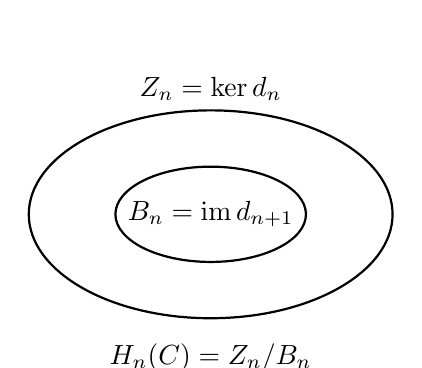
\begin{tikzpicture}[scale=1.1]
	\draw[thick] (0,0) ellipse (2.1 and 1.2);
	\draw[thick] (0,0) ellipse (1.1 and 0.55);
	
	\node at (0,1.45) {$Z_n=\ker d_n$};
	\node at (0,0) {$B_n=\operatorname{im}d_{n+1}$};
	
	\node at (0,-1.65) {$H_n(C)=Z_n/B_n$};
\end{tikzpicture}
\]

If the complex is acyclic, then
\[
H_n(C)=0.
\]
Hence
\[
Z_n=B_n.
\]

So the smaller region fills the whole cycle group.

\subsubsection{Diagram 8.3: Acyclic means exact}

If
\[
H_*(C_\bullet)=0,
\]
then
\[
\ker d_n=\operatorname{im}d_{n+1}
\]
for every \(n\). Therefore the complex is exact:

\[
\begin{tikzcd}[column sep=large]
	\cdots
	\arrow[r]
	&
	C_{n+1}
	\arrow[r,"d_{n+1}"]
	&
	C_n
	\arrow[r,"d_n"]
	&
	C_{n-1}
	\arrow[r,"d_{n-1}"]
	&
	\cdots
	\\
	&
	&
	\ker d_n=\operatorname{im}d_{n+1}
	\arrow[u,hook]
	&
	&
\end{tikzcd}
\]

\subsubsection{Diagram 8.4: Splitting of \(C_n\)}

Because each \(C_n\) is free abelian and the complex is exact, we have a short exact sequence
\[
0\to B_n\to C_n\xrightarrow{d_n} B_{n-1}\to 0.
\]

Since \(B_{n-1}\) is free abelian, the sequence splits. Thus
\[
C_n\cong B_n\oplus A_n.
\]

\[
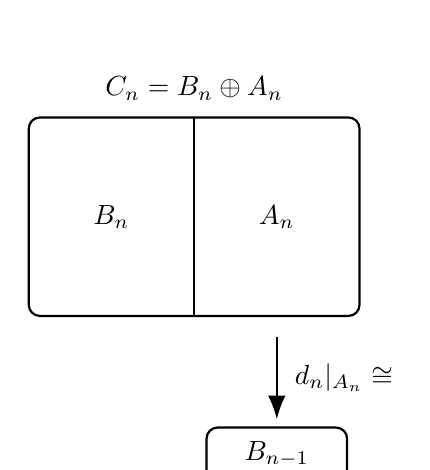
\begin{tikzpicture}[scale=1.05]
	\draw[thick, rounded corners] (-2,-1.2) rectangle (2,1.2);
	\draw[thick] (0,-1.2) -- (0,1.2);
	
	\node at (-1,0) {$B_n$};
	\node at (1,0) {$A_n$};
	\node at (0,1.55) {$C_n=B_n\oplus A_n$};
	
	\draw[-{Latex[length=3mm]}, thick] (1,-1.45) -- (1,-2.45);
	\node[right] at (1.1,-1.95) {$d_n|_{A_n}\cong$};
	
	\draw[thick, rounded corners] (0.15,-3.2) rectangle (1.85,-2.55);
	\node at (1,-2.875) {$B_{n-1}$};
\end{tikzpicture}
\]

The important point is that
\[
d_n|_{A_n}\colon A_n\to B_{n-1}
\]
is an isomorphism.

\subsubsection{Diagram 8.5: Elementary cancellation pair}

Every acyclic free chain complex decomposes into elementary cancellation pieces of the form

\[
\mathbb Z \xrightarrow{\cong} \mathbb Z.
\]

Diagrammatically:

\[
\begin{tikzcd}[column sep=large]
	0
	\arrow[r]
	&
	\mathbb Z
	\arrow[r,"\operatorname{id}"]
	&
	\mathbb Z
	\arrow[r]
	&
	0
\end{tikzcd}
\]

This complex is contractible because the identity map can be undone by a homotopy map going one degree upward.

\[
\begin{tikzcd}[column sep=large,row sep=large]
	C_1=\mathbb Z
	\arrow[r,"d_1=\operatorname{id}"]
	&
	C_0=\mathbb Z
	\arrow[l,bend left=35,"h_0"]
\end{tikzcd}
\]

Here
\[
d_1h_0=\operatorname{id}_{C_0},
\qquad
h_0d_1=\operatorname{id}_{C_1}.
\]

\subsubsection{Diagram 8.6: General contraction formula}

The chain homotopy condition for
\[
\operatorname{id}_{C_\bullet}\simeq 0
\]
is

\[
\operatorname{id}_{C_n}=d_{n+1}h_n+h_{n-1}d_n.
\]

Diagrammatically:

\[
\begin{tikzcd}[column sep=large,row sep=large]
	C_{n+1}
	\arrow[r,"d_{n+1}"]
	&
	C_n
	\arrow[r,"d_n"]
	\arrow[l,bend left=35,"h_n"]
	&
	C_{n-1}
	\arrow[l,bend left=35,"h_{n-1}"]
\end{tikzcd}
\]

The two terms in the formula mean:

\[
d_{n+1}h_n
\]
recovers the boundary part of an element of \(C_n\), while

\[
h_{n-1}d_n
\]
recovers the complementary part.

\subsubsection{Diagram 8.7: Augmented chain complex of an interval}

Let
\[
I=[v_0,v_1].
\]

The augmented chain complex is

\[
0\to C_1(I)\xrightarrow{\partial_1}C_0(I)\xrightarrow{\varepsilon}\mathbb Z\to 0.
\]

\[
\begin{tikzcd}[column sep=large]
	0
	\arrow[r]
	&
	\mathbb Z[e]
	\arrow[r,"\partial_1"]
	&
	\mathbb Z[v_0]\oplus \mathbb Z[v_1]
	\arrow[r,"\varepsilon"]
	&
	\mathbb Z
	\arrow[r]
	&
	0
\end{tikzcd}
\]

where
\[
\partial_1(e)=v_1-v_0,
\]
and
\[
\varepsilon(v_0)=1,
\qquad
\varepsilon(v_1)=1.
\]

Geometrically:

\[
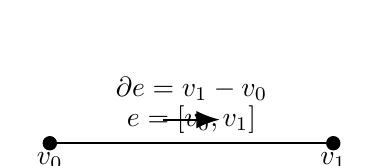
\begin{tikzpicture}[scale=1.2]
	\filldraw (0,0) circle (2pt);
	\filldraw (3,0) circle (2pt);
	
	\draw[thick] (0,0) -- (3,0);
	
	\node[below] at (0,0) {$v_0$};
	\node[below] at (3,0) {$v_1$};
	\node[above] at (1.5,0) {$e=[v_0,v_1]$};
	
	\draw[-{Latex[length=3mm]}, thick] (1.2,0.25) -- (1.8,0.25);
	\node[above] at (1.5,0.35) {$\partial e=v_1-v_0$};
\end{tikzpicture}
\]

The augmentation removes the remaining \(H_0\), making the augmented complex acyclic.

\subsubsection{Chart 8.1: Acyclic and non-acyclic examples}

\[
\begin{array}{c|c|c|c}
	\text{Complex} & H_0 & H_1 & \text{Conclusion} \\
	\hline
	0\to \mathbb Z\xrightarrow{\operatorname{id}}\mathbb Z\to 0
	& 0 & 0 & \text{acyclic and contractible} \\
	\hline
	0\to \mathbb Z\xrightarrow{\times 2}\mathbb Z\to 0
	& \mathbb Z/2\mathbb Z & 0 & \text{not acyclic} \\
	\hline
	0\to \mathbb Z\xrightarrow{n\mapsto(n,n)}\mathbb Z^2
	\xrightarrow{(a,b)\mapsto a-b}\mathbb Z\to 0
	& 0 & 0 & \text{acyclic and contractible}
\end{array}
\]

\subsection{Diagrams for Problem 9: Products of Polyhedra}

\subsubsection{Diagram 9.1: Product of two intervals}

The product
\[
\Delta^1\times\Delta^1
\]
is a square.

\[
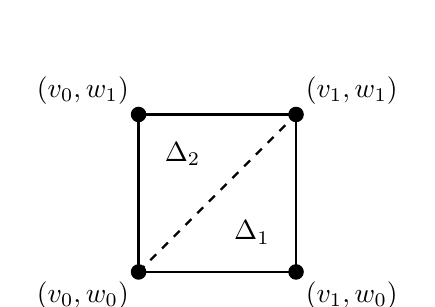
\begin{tikzpicture}[scale=2]
	\coordinate (A) at (0,0);
	\coordinate (B) at (1,0);
	\coordinate (C) at (0,1);
	\coordinate (D) at (1,1);
	
	\draw[thick] (A) -- (B) -- (D) -- (C) -- cycle;
	\draw[thick,dashed] (A) -- (D);
	
	\filldraw (A) circle (1.3pt);
	\filldraw (B) circle (1.3pt);
	\filldraw (C) circle (1.3pt);
	\filldraw (D) circle (1.3pt);
	
	\node[below left] at (A) {$(v_0,w_0)$};
	\node[below right] at (B) {$(v_1,w_0)$};
	\node[above left] at (C) {$(v_0,w_1)$};
	\node[above right] at (D) {$(v_1,w_1)$};
	
	\node at (0.72,0.25) {$\Delta_1$};
	\node at (0.28,0.75) {$\Delta_2$};
\end{tikzpicture}
\]

The square is triangulated into two triangles:

\[
[(v_0,w_0),(v_1,w_0),(v_1,w_1)]
\]

and

\[
[(v_0,w_0),(v_0,w_1),(v_1,w_1)].
\]

\subsubsection{Diagram 9.2: Staircase paths for \(\Delta^1\times\Delta^1\)}

The two triangles correspond to two monotone paths from \((0,0)\) to \((1,1)\).

\[
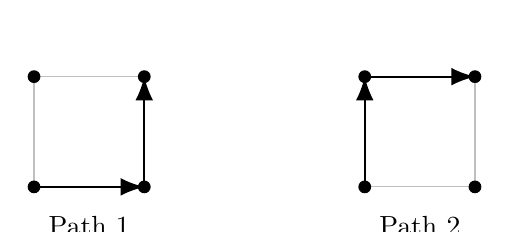
\begin{tikzpicture}[scale=1.4]
	% first grid
	\draw[step=1,gray!50,thin] (0,0) grid (1,1);
	\filldraw (0,0) circle (1.5pt);
	\filldraw (1,0) circle (1.5pt);
	\filldraw (0,1) circle (1.5pt);
	\filldraw (1,1) circle (1.5pt);
	\draw[-{Latex[length=3mm]},thick] (0,0) -- (1,0);
	\draw[-{Latex[length=3mm]},thick] (1,0) -- (1,1);
	\node at (0.5,-0.35) {Path 1};
	
	% second grid
	\begin{scope}[xshift=3cm]
		\draw[step=1,gray!50,thin] (0,0) grid (1,1);
		\filldraw (0,0) circle (1.5pt);
		\filldraw (1,0) circle (1.5pt);
		\filldraw (0,1) circle (1.5pt);
		\filldraw (1,1) circle (1.5pt);
		\draw[-{Latex[length=3mm]},thick] (0,0) -- (0,1);
		\draw[-{Latex[length=3mm]},thick] (0,1) -- (1,1);
		\node at (0.5,-0.35) {Path 2};
	\end{scope}
\end{tikzpicture}
\]

Thus
\[
\Delta^1\times\Delta^1
\]
has
\[
\binom{1+1}{1}=2
\]
maximal simplices.

\subsubsection{Diagram 9.3: Staircase paths for \(\Delta^2\times\Delta^1\)}

For
\[
\Delta^2\times\Delta^1,
\]
the monotone paths go from
\[
(0,0)
\]
to
\[
(2,1).
\]

There are
\[
\binom{2+1}{2}=3
\]
paths.

\[
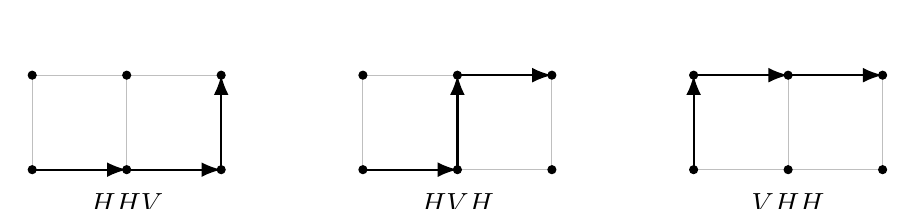
\begin{tikzpicture}[scale=1.2]
	% path 1
	\draw[step=1,gray!50,thin] (0,0) grid (2,1);
	\foreach \x in {0,1,2}{
		\foreach \y in {0,1}{
			\filldraw (\x,\y) circle (1.2pt);
		}
	}
	\draw[-{Latex[length=2.5mm]},thick] (0,0)--(1,0);
	\draw[-{Latex[length=2.5mm]},thick] (1,0)--(2,0);
	\draw[-{Latex[length=2.5mm]},thick] (2,0)--(2,1);
	\node at (1,-0.35) {$HHV$};
	
	% path 2
	\begin{scope}[xshift=3.5cm]
		\draw[step=1,gray!50,thin] (0,0) grid (2,1);
		\foreach \x in {0,1,2}{
			\foreach \y in {0,1}{
				\filldraw (\x,\y) circle (1.2pt);
			}
		}
		\draw[-{Latex[length=2.5mm]},thick] (0,0)--(1,0);
		\draw[-{Latex[length=2.5mm]},thick] (1,0)--(1,1);
		\draw[-{Latex[length=2.5mm]},thick] (1,1)--(2,1);
		\node at (1,-0.35) {$HVH$};
	\end{scope}
	
	% path 3
	\begin{scope}[xshift=7cm]
		\draw[step=1,gray!50,thin] (0,0) grid (2,1);
		\foreach \x in {0,1,2}{
			\foreach \y in {0,1}{
				\filldraw (\x,\y) circle (1.2pt);
			}
		}
		\draw[-{Latex[length=2.5mm]},thick] (0,0)--(0,1);
		\draw[-{Latex[length=2.5mm]},thick] (0,1)--(1,1);
		\draw[-{Latex[length=2.5mm]},thick] (1,1)--(2,1);
		\node at (1,-0.35) {$VHH$};
	\end{scope}
\end{tikzpicture}
\]

Therefore the triangular prism
\[
\Delta^2\times\Delta^1
\]
is triangulated into three tetrahedra.

\subsubsection{Diagram 9.4: Triangular prism from \(\Delta^2\times\Delta^1\)}

\[
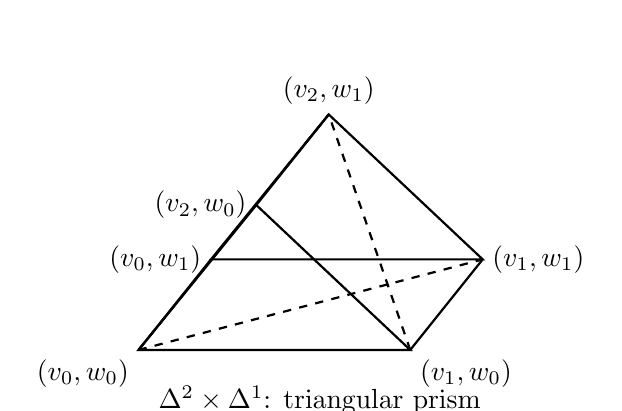
\begin{tikzpicture}[scale=1.15]
	% bottom triangle
	\coordinate (A) at (0,0);
	\coordinate (B) at (3,0);
	\coordinate (C) at (1.3,1.6);
	
	% top triangle shifted
	\coordinate (A2) at (0.8,1.0);
	\coordinate (B2) at (3.8,1.0);
	\coordinate (C2) at (2.1,2.6);
	
	% faces
	\draw[thick] (A)--(B)--(C)--cycle;
	\draw[thick] (A2)--(B2)--(C2)--cycle;
	\draw[thick] (A)--(A2);
	\draw[thick] (B)--(B2);
	\draw[thick] (C)--(C2);
	
	% triangulation diagonals schematic
	\draw[dashed,thick] (A)--(B2);
	\draw[dashed,thick] (A)--(C2);
	\draw[dashed,thick] (B)--(C2);
	
	% labels
	\node[below left] at (A) {$(v_0,w_0)$};
	\node[below right] at (B) {$(v_1,w_0)$};
	\node[left] at (C) {$(v_2,w_0)$};
	
	\node[left] at (A2) {$(v_0,w_1)$};
	\node[right] at (B2) {$(v_1,w_1)$};
	\node[above] at (C2) {$(v_2,w_1)$};
	
	\node at (2,-0.55) {$\Delta^2\times\Delta^1$: triangular prism};
\end{tikzpicture}
\]

The dashed diagonals indicate a possible subdivision into tetrahedra.

\subsubsection{Diagram 9.5: Circle times interval gives a cylinder}

Let \(K\) be a triangulated circle with three edges. Then
\[
|K|\times I
\]
is a cylinder.

One may draw it as a rectangle with the left and right edges identified.

\[
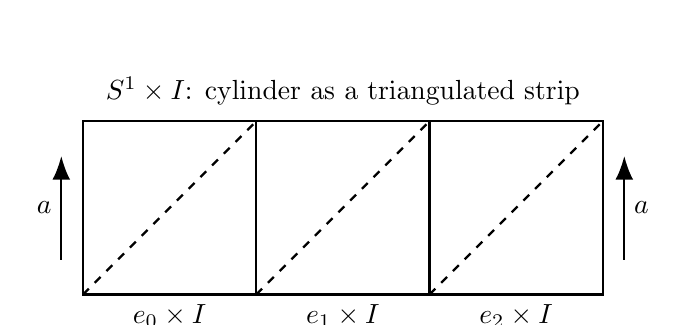
\begin{tikzpicture}[scale=1.1]
	\draw[thick] (0,0) rectangle (6,2);
	
	% vertical subdivisions
	\draw[thick] (2,0)--(2,2);
	\draw[thick] (4,0)--(4,2);
	
	% diagonals
	\draw[dashed,thick] (0,0)--(2,2);
	\draw[dashed,thick] (2,0)--(4,2);
	\draw[dashed,thick] (4,0)--(6,2);
	
	% identification arrows
	\draw[-{Latex[length=3mm]},thick] (-0.25,0.4)--(-0.25,1.6);
	\draw[-{Latex[length=3mm]},thick] (6.25,0.4)--(6.25,1.6);
	
	\node[left] at (-0.25,1) {$a$};
	\node[right] at (6.25,1) {$a$};
	
	\node[below] at (1,0) {$e_0\times I$};
	\node[below] at (3,0) {$e_1\times I$};
	\node[below] at (5,0) {$e_2\times I$};
	
	\node at (3,2.35) {$S^1\times I$: cylinder as a triangulated strip};
\end{tikzpicture}
\]

There are three rectangles, each divided into two triangles. Hence this triangulation has
\[
3\cdot 2=6
\]
triangles.

\subsubsection{Diagram 9.6: Circle times circle gives a torus}

The torus
\[
T^2=S^1\times S^1
\]
can be represented by a square whose opposite edges are identified.

\[
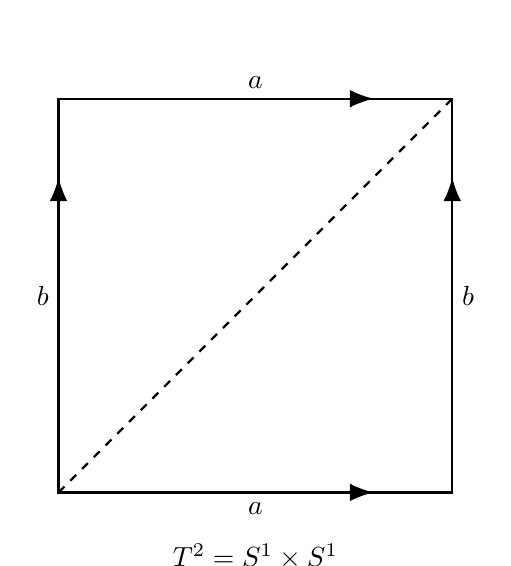
\begin{tikzpicture}[scale=1.25]
	\draw[thick] (0,0) rectangle (4,4);
	
	% diagonal triangulation
	\draw[dashed,thick] (0,0)--(4,4);
	
	% arrows for horizontal identifications
	\draw[-{Latex[length=3mm]},thick] (0.8,0)--(3.2,0);
	\draw[-{Latex[length=3mm]},thick] (0.8,4)--(3.2,4);
	
	% arrows for vertical identifications
	\draw[-{Latex[length=3mm]},thick] (0,0.8)--(0,3.2);
	\draw[-{Latex[length=3mm]},thick] (4,0.8)--(4,3.2);
	
	\node[below] at (2,0) {$a$};
	\node[above] at (2,4) {$a$};
	
	\node[left] at (0,2) {$b$};
	\node[right] at (4,2) {$b$};
	
	\node at (2,-0.65) {$T^2=S^1\times S^1$};
\end{tikzpicture}
\]

This diagram shows the usual quotient-square model of the torus. Product triangulations refine this picture by dividing the square cells into triangles.

\subsubsection{Diagram 9.7: Product construction from cells}

The product of two polyhedra is built from products of simplices:

\[
|K|\times |L|
=
\bigcup_{\sigma\in K,\ \tau\in L}
\sigma\times\tau.
\]

\[
\begin{tikzcd}[column sep=large,row sep=large]
	\sigma\in K
	\arrow[r, "\text{choose}"]
	&
	\sigma\times\tau
	\arrow[r, "\text{triangulate}"]
	&
	\text{simplices in }K\boxtimes L
	\\
	\tau\in L
	\arrow[ur, "\text{choose}"']
	&
	&
\end{tikzcd}
\]

Each product \(\sigma\times\tau\) receives a staircase triangulation.

\subsubsection{Chart 9.1: Simplex products}

\[
\begin{array}{c|c|c|c}
	\text{Product} & \text{Geometric shape} & \text{Dimension} & \text{Maximal simplices} \\
	\hline
	\Delta^0\times\Delta^0
	& \text{point}
	& 0
	& 1
	\\
	\hline
	\Delta^0\times\Delta^1
	& \text{interval}
	& 1
	& 1
	\\
	\hline
	\Delta^1\times\Delta^1
	& \text{square}
	& 2
	& 2
	\\
	\hline
	\Delta^1\times\Delta^2
	& \text{triangular prism}
	& 3
	& 3
	\\
	\hline
	\Delta^2\times\Delta^2
	& \text{4-dimensional product}
	& 4
	& 6
	\\
	\hline
	\Delta^3\times\Delta^1
	& \text{tetrahedral prism}
	& 4
	& 4
\end{array}
\]

In general,
\[
\Delta^p\times\Delta^q
\]
has dimension
\[
p+q
\]
and is triangulated into
\[
\binom{p+q}{p}
\]
maximal simplices.

\subsubsection{Chart 9.2: Shape intuition}

\[
\begin{array}{c|c}
	\text{Product} & \text{Intuition} \\
	\hline
	\text{point}\times X & X \\
	\hline
	\text{interval}\times\text{interval} & \text{square} \\
	\hline
	\text{triangle}\times\text{interval} & \text{triangular prism} \\
	\hline
	S^1\times I & \text{cylinder} \\
	\hline
	S^1\times S^1 & \text{torus} \\
	\hline
	\text{graph}\times I & \text{thickened graph}
\end{array}
\]

\subsection{Final Visual Summary}

\[
\begin{array}{c|c|c}
	\text{Problem} & \text{Main idea} & \text{Visual model} \\
	\hline
	8
	&
	\text{Acyclic free complex}
	&
	\mathbb Z\xrightarrow{\cong}\mathbb Z
	\text{ cancellation pairs}
	\\
	\hline
	9
	&
	\text{Product of polyhedra}
	&
	\Delta^1\times\Delta^1
	=
	\text{square}
	=
	2\text{ triangles}
\end{array}
\]

Problem 8 is algebraic: exactness plus freeness gives splittings and contractions.

Problem 9 is geometric: products of simplices are triangulated by staircase paths, and these triangulations glue together across faces.

\section{Elementary Collapses, Free Faces, and Homology}

\subsection{Main geometric idea}

Let \(K\) be a simplicial complex. Suppose that
\[
\tau \leq \sigma,
\]
where \(\tau\) is a face of \(\sigma\) of codimension \(1\). Thus, if
\[
\dim \sigma=q,
\]
then
\[
\dim \tau=q-1.
\]

Assume that \(\sigma\) is a maximal simplex of \(K\), meaning that \(\sigma\) is not a proper face of any larger simplex in \(K\). Also assume that \(\tau\) is a face of no simplex of \(K\) other than \(\sigma\).

Such a face \(\tau\) is called a \textbf{free face} of \(\sigma\).

We define
\[
L=K\setminus\{\sigma,\tau\}.
\]

The operation
\[
K\searrow L
\]
is called an \textbf{elementary collapse}. Geometrically, we remove one maximal simplex together with one of its free codimension-one faces.

The main result is that this operation does not change homology:
\[
H_j(L)\cong H_j(K)
\]
for every \(j\).

\subsection{Why \(L\) is still a simplicial complex}

We first check that \(L\) is a simplicial complex.

Recall that a simplicial complex must contain all faces of its simplices. Therefore, if
\[
\rho\in L
\]
and
\[
\eta\leq \rho,
\]
then we must show that
\[
\eta\in L.
\]

Since \(L\subset K\), we know that \(\rho\in K\). Because \(K\) is a simplicial complex and \(\eta\leq \rho\), we have
\[
\eta\in K.
\]

The only possible problem is that \(\eta\) might be one of the two simplices removed from \(K\), namely \(\sigma\) or \(\tau\).

First, \(\eta=\sigma\) is impossible. Indeed, \(\eta\leq \rho\), while \(\rho\neq \sigma\), because \(\rho\in L\). A face of \(\rho\) cannot be a larger simplex \(\sigma\).

Second, suppose that
\[
\eta=\tau.
\]
Then
\[
\tau\leq \rho.
\]
But \(\tau\) is assumed to be a face of no simplex of \(K\) other than \(\sigma\). Hence \(\rho=\sigma\), which is impossible because \(\rho\in L\).

Therefore
\[
\eta\neq \sigma,\tau.
\]
So
\[
\eta\in L.
\]

Thus \(L\) is again a simplicial complex.

\subsection{Chain-level description}

Let
\[
i\colon L\hookrightarrow K
\]
be the inclusion. It induces a chain map
\[
i_\bullet\colon C_\bullet(L)\to C_\bullet(K).
\]

Since \(K\) and \(L\) differ only by the two simplices \(\sigma\) and \(\tau\), the chain groups split as follows.

In degree \(q\),
\[
C_q(K)=C_q(L)\oplus \mathbb Z\sigma.
\]

In degree \(q-1\),
\[
C_{q-1}(K)=C_{q-1}(L)\oplus \mathbb Z\tau.
\]

In all other degrees,
\[
C_j(K)=C_j(L)
\qquad
\text{for } j\neq q,q-1.
\]

The key boundary relation is
\[
\partial \sigma=\pm \tau+a,
\]
where
\[
a\in C_{q-1}(L).
\]

After choosing the orientation of \(\sigma\) suitably, we may assume that the coefficient of \(\tau\) is \(+1\). Hence
\[
\partial \sigma=\tau+a.
\]

Here \(a\) is a chain made from the other codimension-one faces of \(\sigma\). These other faces belong to \(L\).

Because
\[
\partial^2=0,
\]
we have
\[
0=\partial^2\sigma=\partial(\tau+a).
\]
Therefore
\[
0=\partial\tau+\partial a.
\]
Hence
\[
\partial\tau=-\partial a.
\]

This identity is the algebraic reason why the elementary collapse preserves homology.

\subsection{Construction of a chain retraction}

We now define a chain map
\[
r_\bullet\colon C_\bullet(K)\to C_\bullet(L)
\]
which behaves like a retraction.

For every simplex \(x\in L\), define
\[
r(x)=x.
\]

For the removed \(q\)-simplex \(\sigma\), define
\[
r(\sigma)=0.
\]

For the removed free face \(\tau\), define
\[
r(\tau)=-a,
\]
where
\[
\partial\sigma=\tau+a.
\]

Thus \(r\) fixes everything in \(L\), kills \(\sigma\), and replaces the free face \(\tau\) by the negative of the remaining boundary of \(\sigma\).

We check that \(r\) is a chain map.

First, for \(\sigma\), we have
\[
r(\partial\sigma)
=
r(\tau+a)
=
r(\tau)+r(a).
\]
Since \(a\in C_{q-1}(L)\), we have \(r(a)=a\). Also \(r(\tau)=-a\). Therefore
\[
r(\partial\sigma)=-a+a=0.
\]
On the other hand,
\[
\partial r(\sigma)=\partial 0=0.
\]
Hence
\[
r\partial\sigma=\partial r\sigma.
\]

Next, for \(\tau\), we have
\[
r(\partial\tau)=\partial\tau,
\]
because \(\partial\tau\in C_{q-2}(L)\). Also,
\[
\partial r(\tau)
=
\partial(-a)
=
-\partial a.
\]
But from
\[
\partial\tau=-\partial a,
\]
we get
\[
\partial r(\tau)=\partial\tau.
\]
Therefore
\[
r\partial\tau=\partial r\tau.
\]

For simplices already in \(L\), the equality
\[
r\partial=\partial r
\]
is immediate, because \(r\) is the identity on \(C_\bullet(L)\).

Thus \(r_\bullet\) is a chain map.

Moreover,
\[
r_\bullet i_\bullet=\operatorname{id}_{C_\bullet(L)}.
\]

So \(r_\bullet\) is a left inverse of the inclusion on the chain level.

\subsection{Chain homotopy between \(i r\) and the identity}

We now show that
\[
i_\bullet r_\bullet
\]
is chain homotopic to
\[
\operatorname{id}_{C_\bullet(K)}.
\]

Define homomorphisms
\[
h_j\colon C_j(K)\to C_{j+1}(K)
\]
by
\[
h(\tau)=\sigma
\]
and
\[
h(x)=0
\]
for every other basis simplex \(x\).

We claim that
\[
\operatorname{id}_{C_\bullet(K)}-i_\bullet r_\bullet
=
\partial h+h\partial.
\]

We check this on basis simplices.

First, consider \(\sigma\). Since
\[
r(\sigma)=0,
\]
we get
\[
(\operatorname{id}-ir)(\sigma)=\sigma.
\]
On the other hand,
\[
(\partial h+h\partial)(\sigma)
=
\partial h(\sigma)+h(\partial\sigma).
\]
Because
\[
h(\sigma)=0
\]
and
\[
\partial\sigma=\tau+a,
\]
we have
\[
h(\partial\sigma)
=
h(\tau+a)
=
h(\tau)+h(a).
\]
Since \(a\in C_{q-1}(L)\), we have \(h(a)=0\). Therefore
\[
h(\partial\sigma)=\sigma.
\]
Thus
\[
(\partial h+h\partial)(\sigma)=\sigma.
\]

So the formula holds on \(\sigma\).

Now consider \(\tau\). Since
\[
r(\tau)=-a,
\]
we get
\[
(\operatorname{id}-ir)(\tau)
=
\tau-ir(\tau)
=
\tau-(-a)
=
\tau+a.
\]
On the other hand,
\[
(\partial h+h\partial)(\tau)
=
\partial h(\tau)+h(\partial\tau).
\]
Since
\[
h(\tau)=\sigma,
\]
we get
\[
\partial h(\tau)=\partial\sigma=\tau+a.
\]
Also, \(\partial\tau\in C_{q-2}(L)\), so
\[
h(\partial\tau)=0.
\]
Therefore
\[
(\partial h+h\partial)(\tau)=\tau+a.
\]

So the formula holds on \(\tau\).

Finally, let \(x\in L\). Since \(r(x)=x\), we have
\[
(\operatorname{id}-ir)(x)=x-x=0.
\]
Also, \(h(x)=0\). Since \(L\) is a subcomplex, \(\partial x\in C_\bullet(L)\), so
\[
h(\partial x)=0.
\]
Thus
\[
(\partial h+h\partial)(x)=0.
\]

Therefore
\[
\operatorname{id}_{C_\bullet(K)}-i_\bullet r_\bullet
=
\partial h+h\partial.
\]

Hence
\[
i_\bullet r_\bullet\simeq \operatorname{id}_{C_\bullet(K)}.
\]

Together with
\[
r_\bullet i_\bullet=\operatorname{id}_{C_\bullet(L)},
\]
this shows that
\[
C_\bullet(K)
\]
and
\[
C_\bullet(L)
\]
are chain homotopy equivalent.

Therefore
\[
H_j(K)\cong H_j(L)
\]
for every \(j\).

\subsection{Relative homology viewpoint}

There is also a shorter proof using relative homology.

Consider the relative chain complex
\[
C_\bullet(K,L)=C_\bullet(K)/C_\bullet(L).
\]

Since \(K\) and \(L\) differ only by \(\sigma\) and \(\tau\), the quotient complex has only two nonzero groups:
\[
C_q(K,L)\cong \mathbb Z[\sigma],
\]
and
\[
C_{q-1}(K,L)\cong \mathbb Z[\tau].
\]

The boundary map is
\[
\partial[\sigma]=\pm[\tau].
\]

Thus the relative chain complex is of the form
\[
0\longrightarrow \mathbb Z
\xrightarrow{\cong}
\mathbb Z
\longrightarrow 0.
\]

This complex is acyclic. Therefore
\[
H_j(K,L)=0
\]
for every \(j\).

Now use the long exact sequence of the pair \((K,L)\):
\[
\cdots
\longrightarrow H_j(L)
\xrightarrow{i_*}
H_j(K)
\longrightarrow H_j(K,L)
\longrightarrow H_{j-1}(L)
\longrightarrow \cdots .
\]

Since
\[
H_j(K,L)=0
\]
for all \(j\), the map
\[
i_*\colon H_j(L)\to H_j(K)
\]
is an isomorphism for every \(j\).

Therefore elementary collapse preserves homology.

\subsection{Example 1: A filled triangle collapses to two edges}

Let
\[
K=\Delta^2
\]
be a filled triangle.

Choose one boundary edge \(\tau\), and let
\[
\sigma=\Delta^2.
\]

The edge \(\tau\) is a free face because it belongs only to the triangle \(\sigma\).

Now remove both:
\[
L=K\setminus\{\sigma,\tau\}.
\]

What remains is two edges meeting at one vertex. This space is shaped like the letter \(V\), so it is contractible.

Therefore \(K\) and \(L\) have the same homology:
\[
H_0(K)\cong H_0(L)\cong \mathbb Z,
\]
and
\[
H_j(K)\cong H_j(L)=0
\qquad
\text{for } j\geq 1.
\]

The elementary collapse removes no genuine hole.

\subsection{Example 2: A tetrahedron collapses by removing one face}

Let
\[
K=\Delta^3
\]
be a filled tetrahedron.

Take
\[
\sigma=\Delta^3,
\]
and let \(\tau\) be one triangular face of \(\sigma\).

The face \(\tau\) is free because it belongs only to the tetrahedron \(\sigma\).

Removing \(\sigma\) and \(\tau\) leaves the other three triangular faces. This remaining complex is still contractible, geometrically like a disk.

Hence
\[
H_0(K)\cong \mathbb Z,
\]
and
\[
H_j(K)=0
\qquad
\text{for } j\geq 1.
\]

The same homology groups are obtained for the collapsed complex \(L\).

\subsection{Example 3: A triangulated disk}

Suppose \(K\) is a triangulated disk.

Usually, a triangle at the boundary has a boundary edge that belongs only to that triangle. Such an edge is a free face.

We may remove that triangle together with the free edge. Then we repeat this process.

In many triangulations of a disk, repeated elementary collapses reduce the whole complex to a single vertex:
\[
K\searrow \{\text{point}\}.
\]

Therefore a triangulated disk has the same homology as a point:
\[
H_0(K)\cong \mathbb Z,
\]
and
\[
H_j(K)=0
\qquad
\text{for } j\geq 1.
\]

This matches the geometric intuition that a disk is connected and has no holes.

\subsection{Example 4: A circle has no free face}

Let \(K\) be a triangulated circle.

In a one-dimensional simplicial complex, an elementary collapse removes an edge together with a free vertex.

But in a circle, every vertex belongs to two edges. Therefore no vertex is free.

Hence a triangulated circle has no elementary collapse of this type.

The homology of the circle is
\[
H_0(S^1)\cong \mathbb Z,
\]
\[
H_1(S^1)\cong \mathbb Z,
\]
and
\[
H_j(S^1)=0
\qquad
\text{for } j\geq 2.
\]

The generator of \(H_1(S^1)\) is represented by the cycle going once around the circle.

This example shows that elementary collapses cannot remove genuine holes.

\subsection{How collapses help compute homology}

Elementary collapses are useful because they simplify a complex without changing its homology.

The general strategy is:
\[
\text{complicated complex}
\quad
\searrow
\quad
\text{simpler complex}
\quad
\searrow
\quad
\text{minimal core}.
\]

Since every elementary collapse preserves homology, we may compute the homology of the final simplified complex instead of the original one.

Typical outcomes are as follows.

If a complex collapses to a point, then
\[
H_0\cong \mathbb Z,
\]
and
\[
H_j=0
\qquad
\text{for } j\geq 1.
\]

If a complex collapses to a circle \(S^1\), then
\[
H_0\cong \mathbb Z,
\]
\[
H_1\cong \mathbb Z,
\]
and
\[
H_j=0
\qquad
\text{for } j\geq 2.
\]

If a complex collapses to a wedge of two circles
\[
S^1\vee S^1,
\]
then
\[
H_0\cong \mathbb Z,
\]
\[
H_1\cong \mathbb Z^2,
\]
and
\[
H_j=0
\qquad
\text{for } j\geq 2.
\]

If a complex collapses to a sphere \(S^2\), then
\[
H_0\cong \mathbb Z,
\]
\[
H_2\cong \mathbb Z,
\]
and
\[
H_j=0
\qquad
\text{for } j\neq 0,2.
\]

If a complex collapses to a torus \(T^2\), then
\[
H_0\cong \mathbb Z,
\]
\[
H_1\cong \mathbb Z^2,
\]
\[
H_2\cong \mathbb Z,
\]
and
\[
H_j=0
\qquad
\text{for } j\geq 3.
\]

\subsection{How to describe homology generators}

After simplifying a complex by collapses, the generators of homology are described by the remaining cycles.

For \(H_0\), a generator is represented by a vertex in each connected component. If the complex is connected, then
\[
H_0\cong \mathbb Z
\]
with generator represented by any vertex
\[
[v].
\]

For \(H_1\), a generator is represented by a loop of edges. For example, in a triangulated circle,
\[
e_1+e_2+\cdots+e_n
\]
represents a generator of
\[
H_1(S^1)\cong \mathbb Z.
\]

For \(H_2\), a generator is represented by a closed oriented surface. For example, in a triangulated sphere,
\[
\sum_i \pm \sigma_i
\]
where the sum is taken over all oriented triangular faces, represents a generator of
\[
H_2(S^2)\cong \mathbb Z.
\]

For a torus,
\[
H_1(T^2)\cong \mathbb Z^2.
\]
The two generators are represented by two fundamental loops:
\[
a=\text{loop around one direction},
\]
and
\[
b=\text{loop around the other direction}.
\]

Also,
\[
H_2(T^2)\cong \mathbb Z
\]
is generated by the oriented sum of all triangular faces of the torus.

\subsection{Core intuition}

An elementary collapse removes a pair
\[
(\sigma,\tau),
\]
where \(\sigma\) is a simplex and \(\tau\) is a free codimension-one face of \(\sigma\).

Algebraically, this pair behaves like a cancellation pair:
\[
\mathbb Z[\sigma]
\xrightarrow{\partial}
\mathbb Z[\tau].
\]

Since
\[
\partial\sigma=\pm\tau+\text{terms already in }L,
\]
the simplex \(\sigma\) kills the face \(\tau\) exactly. Removing both does not remove any genuine cycle and does not create any new boundary.

Thus the main slogan is:
\[
\boxed{
	\text{Free faces can be collapsed without changing homology.}
}
\]

Elementary collapses are powerful because they reduce complicated simplicial complexes to much simpler ones while preserving all homology groups.

\section{Examples of Elementary Collapses}

In this section we give simple, medium, and harder examples of elementary collapses and their effect on homology.

Recall the situation:
\[
K\searrow L=K\setminus\{\sigma,\tau\},
\]
where \(\sigma\) is a maximal simplex of \(K\), and \(\tau\leq \sigma\) is a free codimension-one face of \(\sigma\).

The main theorem says that the inclusion
\[
i\colon L\hookrightarrow K
\]
induces isomorphisms
\[
i_*\colon H_j(L)\xrightarrow{\cong}H_j(K)
\]
for every \(j\).

Thus elementary collapses preserve homology.

\subsection{Simple Examples}

\subsubsection{Example 1.1: An interval collapses to a point}

Let
\[
K=[v_0,v_1]
\]
be one closed edge.

The simplices of \(K\) are
\[
[v_0],\qquad [v_1],\qquad [v_0,v_1].
\]

Take
\[
\sigma=[v_0,v_1],
\qquad
\tau=[v_1].
\]

The vertex \([v_1]\) is a free face because it belongs only to the edge \([v_0,v_1]\).

Remove both:
\[
L=K\setminus\{[v_0,v_1],[v_1]\}.
\]

Then
\[
L=\{[v_0]\}.
\]

Hence
\[
[v_0,v_1]\searrow [v_0].
\]

Before the collapse, \(K\) is an interval, so it is contractible. Therefore
\[
H_0(K)\cong \mathbb Z,
\]
and
\[
H_j(K)=0
\qquad
\text{for }j\geq 1.
\]

After the collapse, \(L\) is a single point, so
\[
H_0(L)\cong \mathbb Z,
\]
and
\[
H_j(L)=0
\qquad
\text{for }j\geq 1.
\]

Thus the collapse preserves homology.

\subsubsection{Example 1.2: A filled triangle collapses to two edges}

Let
\[
K=\Delta^2=[v_0,v_1,v_2]
\]
be a filled triangle.

Choose
\[
\sigma=[v_0,v_1,v_2],
\qquad
\tau=[v_1,v_2].
\]

The edge \([v_1,v_2]\) belongs only to the triangle \([v_0,v_1,v_2]\), so it is a free face.

Remove both:
\[
L=K\setminus\{[v_0,v_1,v_2],[v_1,v_2]\}.
\]

What remains is
\[
[v_0,v_1]\cup [v_0,v_2].
\]

Geometrically, this is shaped like the letter \(V\). Hence
\[
\Delta^2\searrow [v_0,v_1]\cup [v_0,v_2].
\]

The filled triangle and the \(V\)-shape are both contractible. Therefore
\[
H_0(K)\cong H_0(L)\cong \mathbb Z,
\]
and
\[
H_j(K)\cong H_j(L)=0
\qquad
\text{for }j\geq 1.
\]

\subsubsection{Example 1.3: The \(V\)-shape collapses to a point}

Now take the remaining complex
\[
L=[v_0,v_1]\cup [v_0,v_2].
\]

Choose
\[
\sigma=[v_0,v_1],
\qquad
\tau=[v_1].
\]

The vertex \([v_1]\) is free because it belongs only to the edge \([v_0,v_1]\).

Remove both:
\[
L_1=L\setminus\{[v_0,v_1],[v_1]\}.
\]

Then
\[
L_1=[v_0,v_2].
\]

Now choose
\[
\sigma=[v_0,v_2],
\qquad
\tau=[v_2].
\]

The vertex \([v_2]\) is a free face of the edge \([v_0,v_2]\). Remove both:
\[
L_2=L_1\setminus\{[v_0,v_2],[v_2]\}.
\]

Then
\[
L_2=\{[v_0]\}.
\]

Thus the filled triangle collapses all the way to a point:
\[
\Delta^2
\searrow
[v_0,v_1]\cup[v_0,v_2]
\searrow
[v_0,v_2]
\searrow
[v_0].
\]

Therefore
\[
\Delta^2\searrow \{\text{point}\}.
\]

Hence
\[
H_0(\Delta^2)\cong \mathbb Z,
\]
and
\[
H_j(\Delta^2)=0
\qquad
\text{for }j\geq 1.
\]

\subsection{Medium Examples}

\subsubsection{Example 2.1: A square divided into two triangles collapses to a point}

Let \(K\) be a square triangulated by one diagonal.

Let the vertices be
\[
v_0,v_1,v_2,v_3,
\]
and suppose the square is divided into the two triangles
\[
[v_0,v_1,v_2]
\]
and
\[
[v_0,v_2,v_3].
\]

Thus
\[
K=[v_0,v_1,v_2]\cup [v_0,v_2,v_3].
\]

The diagonal is
\[
[v_0,v_2].
\]

Since \(K\) is a filled square, it should collapse to a point.

First choose
\[
\sigma_1=[v_0,v_1,v_2],
\qquad
\tau_1=[v_1,v_2].
\]

The edge \([v_1,v_2]\) is a boundary edge and belongs only to \(\sigma_1\), so it is a free face.

Remove both:
\[
K_1=K\setminus\{\sigma_1,\tau_1\}.
\]

Now choose
\[
\sigma_2=[v_0,v_2,v_3],
\qquad
\tau_2=[v_2,v_3].
\]

The edge \([v_2,v_3]\) is now free.

Remove both:
\[
K_2=K_1\setminus\{\sigma_2,\tau_2\}.
\]

What remains is a tree of edges, for example
\[
[v_0,v_1]\cup [v_0,v_2]\cup [v_0,v_3].
\]

A tree collapses to a point by repeatedly removing a leaf edge and its leaf vertex.

Therefore
\[
K\searrow \{\text{point}\}.
\]

Hence
\[
H_0(K)\cong \mathbb Z,
\]
and
\[
H_j(K)=0
\qquad
\text{for }j\geq 1.
\]

\subsubsection{Example 2.2: A triangulated disk collapses to a point}

Let \(K\) be a triangulated disk.

For example, imagine a polygon cut into many triangles. A boundary triangle usually has at least one boundary edge that belongs only to that triangle. Such an edge is a free face.

Thus we can remove a pair of the form
\[
(\text{boundary triangle},\text{free boundary edge}).
\]

After removing one such pair, we obtain a smaller triangulated disk or a smaller contractible complex. We then repeat the process.

Each elementary collapse removes one triangle and one free edge.

Eventually, a collapsible triangulated disk reduces to a graph. Since a disk has no essential loop, the remaining graph can be reduced to a tree, and the tree collapses to a point.

Thus, for a collapsible triangulated disk,
\[
K\searrow \{\text{point}\}.
\]

Therefore
\[
H_0(K)\cong \mathbb Z,
\]
and
\[
H_j(K)=0
\qquad
\text{for }j\geq 1.
\]

This is a central example: disks are homologically trivial except in degree \(0\).

\subsubsection{Example 2.3: A tree collapses to a point}

Let \(K\) be a finite tree.

A tree is a connected graph with no cycles.

Every finite tree has at least one leaf vertex. A leaf vertex is a vertex that belongs to exactly one edge.

Let \(v\) be a leaf vertex, and let
\[
e=[v,w]
\]
be the unique edge containing \(v\).

Then
\[
\tau=[v]
\]
is a free face of
\[
\sigma=e.
\]

Remove both:
\[
K_1=K\setminus\{e,v\}.
\]

The result is again a tree, unless the original tree was just one edge.

Repeating this process, every finite tree collapses to a point:
\[
K\searrow \{\text{point}\}.
\]

Therefore
\[
H_0(K)\cong \mathbb Z,
\]
and
\[
H_1(K)=0.
\]

This example is important because it shows that collapses detect the absence of loops in a graph.

\subsubsection{Example 2.4: A circle does not collapse to a point}

Let \(K\) be a triangulated circle with vertices
\[
v_0,v_1,v_2
\]
and edges
\[
[v_0,v_1],
\qquad
[v_1,v_2],
\qquad
[v_2,v_0].
\]

In a graph, an elementary collapse removes an edge together with a free vertex.

But every vertex of a circle belongs to two edges. Therefore there is no free vertex.

Hence a triangulated circle has no elementary collapse.

Its homology is
\[
H_0(S^1)\cong \mathbb Z,
\]
\[
H_1(S^1)\cong \mathbb Z,
\]
and
\[
H_j(S^1)=0
\qquad
\text{for }j\geq 2.
\]

The nonzero group \(H_1(S^1)\) corresponds to the loop going once around the circle.

This example shows that genuine holes cannot be removed by elementary collapses.

\subsection{Harder Examples}

\subsubsection{Example 3.1: An annulus collapses to a circle}

Let \(K\) be a triangulated annulus.

Geometrically, an annulus is a cylinder-like band:
\[
S^1\times [0,1].
\]

It has one essential circular hole.

By elementary collapses, one can remove triangles from the boundary of the annulus, peeling off layers, until the annulus collapses to its central circle:
\[
K\searrow S^1.
\]

Therefore
\[
H_0(K)\cong \mathbb Z,
\]
\[
H_1(K)\cong \mathbb Z,
\]
and
\[
H_j(K)=0
\qquad
\text{for }j\geq 2.
\]

The collapse cannot remove the central loop, because that loop represents a genuine \(H_1\)-class.

Thus the annulus is not collapsible to a point, but it collapses to a circle.

\subsubsection{Example 3.2: A solid tetrahedron collapses to a point}

Let
\[
K=\Delta^3=[v_0,v_1,v_2,v_3]
\]
be a filled tetrahedron.

Choose one triangular face, for example
\[
\tau=[v_1,v_2,v_3].
\]

This is a free face of the tetrahedron
\[
\sigma=[v_0,v_1,v_2,v_3].
\]

Remove both:
\[
K_1=K\setminus\{\sigma,\tau\}.
\]

Now \(K_1\) consists of the other three triangular faces:
\[
[v_0,v_1,v_2],
\qquad
[v_0,v_1,v_3],
\qquad
[v_0,v_2,v_3].
\]

This remaining complex is like a triangular disk made of three triangles. It collapses further to a tree and then to a point.

Therefore
\[
\Delta^3\searrow \{\text{point}\}.
\]

So
\[
H_0(\Delta^3)\cong \mathbb Z,
\]
and
\[
H_j(\Delta^3)=0
\qquad
\text{for }j\geq 1.
\]

This is the three-dimensional analogue of the filled triangle.

\subsubsection{Example 3.3: The boundary of a tetrahedron does not collapse to a point}

Now let \(K\) be not the filled tetrahedron, but only its boundary:
\[
K=\partial \Delta^3.
\]

This is a triangulated sphere:
\[
\partial \Delta^3\cong S^2.
\]

It consists of four triangular faces:
\[
[v_1,v_2,v_3],
\]
\[
[v_0,v_2,v_3],
\]
\[
[v_0,v_1,v_3],
\]
and
\[
[v_0,v_1,v_2].
\]

Every edge belongs to exactly two triangles.

Therefore no edge is a free face of a triangle. Hence there is no elementary collapse of dimension \(2\).

This reflects the fact that \(S^2\) has genuine \(2\)-dimensional homology:
\[
H_0(S^2)\cong \mathbb Z,
\]
\[
H_2(S^2)\cong \mathbb Z,
\]
and
\[
H_1(S^2)=0.
\]

The group \(H_2(S^2)\) is generated by the oriented sum of all triangular faces.

So the boundary of a tetrahedron cannot collapse to a point because it contains a closed surface cycle.

\subsubsection{Example 3.4: A torus cannot collapse to a point}

Let \(K\) be a triangulated torus:
\[
K\cong T^2.
\]

The torus has homology
\[
H_0(T^2)\cong \mathbb Z,
\]
\[
H_1(T^2)\cong \mathbb Z^2,
\]
\[
H_2(T^2)\cong \mathbb Z.
\]

The group \(H_1(T^2)\) has two independent generators:
\[
a=\text{meridian loop},
\]
and
\[
b=\text{longitude loop}.
\]

The group \(H_2(T^2)\) is generated by the oriented sum of all triangular faces.

If the torus collapsed to a point, then it would have the same homology as a point:
\[
H_0\cong \mathbb Z,
\]
and
\[
H_j=0
\qquad
\text{for }j\geq 1.
\]

But the torus has nonzero \(H_1\) and nonzero \(H_2\). Therefore a triangulated torus cannot collapse to a point.

This example shows how homology obstructs collapsibility.

\subsubsection{Example 3.5: A cone collapses to its apex}

Let \(A\) be a simplicial complex, and let
\[
K=\operatorname{Cone}(A)
\]
be the cone on \(A\).

This means we add a new vertex \(p\), called the apex, and join \(p\) to every simplex of \(A\).

For example:
\[
\operatorname{Cone}(S^1)
\]
is a disk, and
\[
\operatorname{Cone}(S^2)
\]
is a ball.

Cones are always contractible. In many finite simplicial cases, a cone can be collapsed to its apex:
\[
\operatorname{Cone}(A)\searrow \{p\}.
\]

Therefore
\[
H_0(\operatorname{Cone}(A))\cong \mathbb Z,
\]
and
\[
H_j(\operatorname{Cone}(A))=0
\qquad
\text{for }j\geq 1.
\]

This is a powerful example because it explains why attaching a cone kills homology.

For instance, \(S^1\) has a nontrivial loop:
\[
H_1(S^1)\cong \mathbb Z.
\]

But the cone over \(S^1\) fills this loop with a disk. Therefore
\[
H_1(\operatorname{Cone}(S^1))=0.
\]

\subsection{Hard Algebraic Example: Collapse as Chain Cancellation}

Let \(K\) be a simplicial complex with a simplex \(\sigma\) and a free face \(\tau\), where
\[
\dim \sigma=q,
\qquad
\dim \tau=q-1.
\]

Let
\[
L=K\setminus\{\sigma,\tau\}.
\]

Suppose that, after choosing orientations,
\[
\partial\sigma=\tau+a,
\]
where
\[
a\in C_{q-1}(L).
\]

Then the relative chain complex
\[
C_\bullet(K,L)
\]
has only two nonzero groups:
\[
C_q(K,L)=\mathbb Z[\sigma],
\]
and
\[
C_{q-1}(K,L)=\mathbb Z[\tau].
\]

The boundary map is
\[
\partial[\sigma]=[\tau].
\]

Thus \(C_\bullet(K,L)\) has the form
\[
0\longrightarrow \mathbb Z[\sigma]
\xrightarrow{\cong}
\mathbb Z[\tau]
\longrightarrow 0.
\]

This complex is acyclic, so
\[
H_j(K,L)=0
\qquad
\text{for all }j.
\]

Now consider the long exact sequence of the pair \((K,L)\):
\[
\cdots
\longrightarrow H_j(L)
\xrightarrow{i_*}
H_j(K)
\longrightarrow H_j(K,L)
\longrightarrow H_{j-1}(L)
\longrightarrow \cdots .
\]

Since
\[
H_j(K,L)=0
\]
for all \(j\), it follows that
\[
i_*\colon H_j(L)\to H_j(K)
\]
is an isomorphism for every \(j\).

Thus an elementary collapse is exactly the removal of an acyclic two-term summand:
\[
\mathbb Z[\sigma]\xrightarrow{\cong}\mathbb Z[\tau].
\]

\subsection{Summary Chart}

\[
\begin{array}{c|c|c|c}
	\text{Complex} & \text{Collapse result} & \text{Homology} & \text{Difficulty} \\
	\hline
	\text{interval}
	&
	\text{point}
	&
	H_0\cong \mathbb Z
	&
	\text{simple}
	\\
	\hline
	\text{filled triangle}
	&
	\text{point}
	&
	H_0\cong \mathbb Z
	&
	\text{simple}
	\\
	\hline
	\text{tree}
	&
	\text{point}
	&
	H_0\cong \mathbb Z
	&
	\text{medium}
	\\
	\hline
	\text{circle}
	&
	\text{no collapse to point}
	&
	H_0\cong \mathbb Z,\ H_1\cong \mathbb Z
	&
	\text{medium}
	\\
	\hline
	\text{annulus}
	&
	\text{circle}
	&
	H_0\cong \mathbb Z,\ H_1\cong \mathbb Z
	&
	\text{harder}
	\\
	\hline
	\text{filled tetrahedron}
	&
	\text{point}
	&
	H_0\cong \mathbb Z
	&
	\text{harder}
	\\
	\hline
	\partial\Delta^3\cong S^2
	&
	\text{no collapse to point}
	&
	H_0\cong \mathbb Z,\ H_2\cong \mathbb Z
	&
	\text{harder}
	\\
	\hline
	T^2
	&
	\text{no collapse to point}
	&
	H_0\cong \mathbb Z,\ H_1\cong \mathbb Z^2,\ H_2\cong \mathbb Z
	&
	\text{hard}
\end{array}
\]

\subsection{Key Intuition}

An elementary collapse removes a pair
\[
(\sigma,\tau),
\]
where \(\sigma\) is a simplex and \(\tau\) is a free codimension-one face of \(\sigma\).

This pair contributes only an acyclic chain piece:
\[
\mathbb Z[\sigma]\xrightarrow{\cong}\mathbb Z[\tau].
\]

Therefore removing this pair does not change homology.

However, genuine loops and closed surfaces cannot be removed this way. This is why
\[
\text{a disk collapses to a point},
\]
but
\[
S^1
\]
does not collapse to a point, and
\[
S^2
\]
does not collapse to a point.

The main rule is:
\[
\boxed{
	\text{Collapses remove contractible pieces, not genuine holes.}
}
\]

\section{Diagrams and Charts for Elementary Collapses}

\subsection{Diagram 1: Free face and elementary collapse}

An elementary collapse removes a maximal simplex \(\sigma\) together with a free codimension-one face \(\tau\):

\[
K\searrow L=K\setminus\{\sigma,\tau\}.
\]

\[
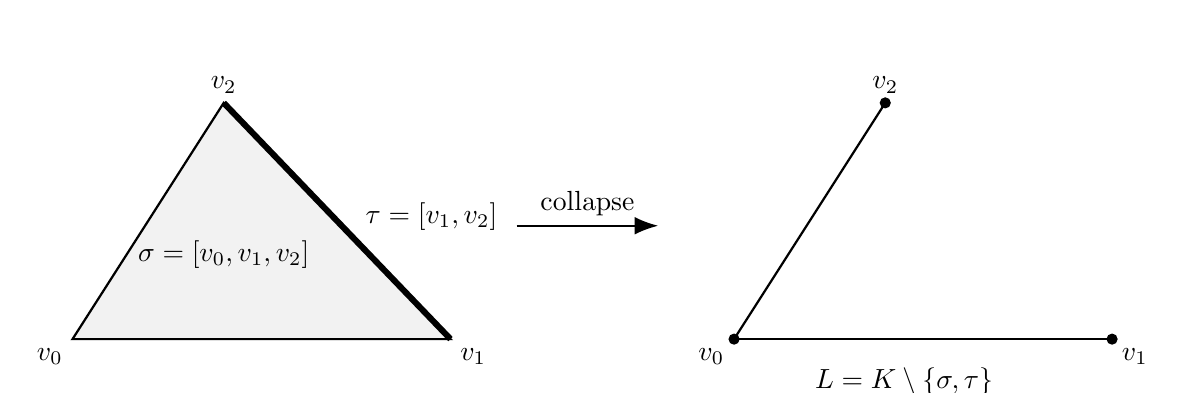
\begin{tikzpicture}[scale=1.2]
	% triangle
	\coordinate (A) at (0,0);
	\coordinate (B) at (4,0);
	\coordinate (C) at (1.6,2.5);
	
	\fill[gray!10] (A)--(B)--(C)--cycle;
	\draw[thick] (A)--(B)--(C)--cycle;
	
	% free edge
	\draw[line width=2.2pt] (B)--(C);
	
	\node[below left] at (A) {$v_0$};
	\node[below right] at (B) {$v_1$};
	\node[above] at (C) {$v_2$};
	
	\node at (1.6,0.9) {$\sigma=[v_0,v_1,v_2]$};
	\node[right] at (3.0,1.3) {$\tau=[v_1,v_2]$};
	
	\draw[-{Latex[length=3mm]},thick] (4.7,1.2)--(6.2,1.2);
	\node[above] at (5.45,1.2) {$\text{collapse}$};
	
	% after collapse V shape
	\coordinate (A2) at (7,0);
	\coordinate (B2) at (11,0);
	\coordinate (C2) at (8.6,2.5);
	
	\draw[thick] (A2)--(B2);
	\draw[thick] (A2)--(C2);
	\filldraw (A2) circle (1.5pt);
	\filldraw (B2) circle (1.5pt);
	\filldraw (C2) circle (1.5pt);
	
	\node[below left] at (A2) {$v_0$};
	\node[below right] at (B2) {$v_1$};
	\node[above] at (C2) {$v_2$};
	
	\node at (8.8,-0.45) {$L=K\setminus\{\sigma,\tau\}$};
\end{tikzpicture}
\]

The edge \(\tau\) is free because it belongs only to the triangle \(\sigma\). Removing both does not change homology.

\subsection{Diagram 2: Interval collapses to a point}

\[
[v_0,v_1]\searrow [v_0].
\]

\[
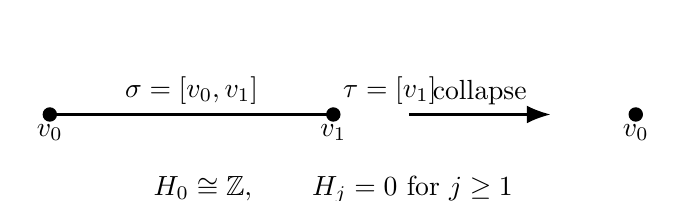
\begin{tikzpicture}[scale=1.2]
	\coordinate (A) at (0,0);
	\coordinate (B) at (3,0);
	
	\draw[thick] (A)--(B);
	\filldraw (A) circle (2pt);
	\filldraw (B) circle (2pt);
	
	\node[below] at (A) {$v_0$};
	\node[below] at (B) {$v_1$};
	\node[above] at (1.5,0) {$\sigma=[v_0,v_1]$};
	\node[above right] at (B) {$\tau=[v_1]$};
	
	\draw[-{Latex[length=3mm]},thick] (3.8,0)--(5.3,0);
	\node[above] at (4.55,0) {$\text{collapse}$};
	
	\coordinate (C) at (6.2,0);
	\filldraw (C) circle (2pt);
	\node[below] at (C) {$v_0$};
	
	\node at (3,-0.8) {$H_0\cong \mathbb Z,\qquad H_j=0\text{ for }j\geq 1$};
\end{tikzpicture}
\]

\subsection{Diagram 3: Filled triangle collapses to a point}

A filled triangle collapses by removing a triangle with a free edge, then removing leaf edges.

\[
\Delta^2
\searrow
\text{\(V\)-shape}
\searrow
\text{edge}
\searrow
\text{point}.
\]

\[
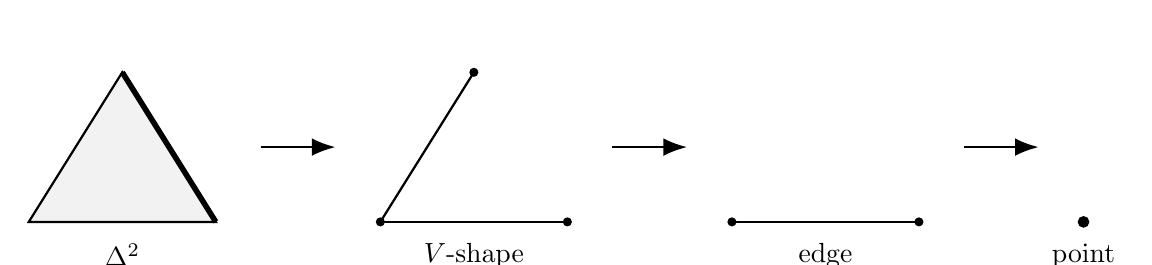
\begin{tikzpicture}[scale=0.95]
	% Stage 1: filled triangle
	\coordinate (A) at (0,0);
	\coordinate (B) at (2.5,0);
	\coordinate (C) at (1.25,2);
	
	\fill[gray!10] (A)--(B)--(C)--cycle;
	\draw[thick] (A)--(B)--(C)--cycle;
	\draw[line width=2pt] (B)--(C);
	\node at (1.25,-0.45) {$\Delta^2$};
	
	% arrow
	\draw[-{Latex[length=3mm]},thick] (3.1,1)--(4.1,1);
	
	% Stage 2: V
	\begin{scope}[xshift=4.7cm]
		\coordinate (A) at (0,0);
		\coordinate (B) at (2.5,0);
		\coordinate (C) at (1.25,2);
		\draw[thick] (A)--(B);
		\draw[thick] (A)--(C);
		\filldraw (A) circle (1.5pt);
		\filldraw (B) circle (1.5pt);
		\filldraw (C) circle (1.5pt);
		\node at (1.25,-0.45) {\(V\)-shape};
	\end{scope}
	
	% arrow
	\draw[-{Latex[length=3mm]},thick] (7.8,1)--(8.8,1);
	
	% Stage 3: edge
	\begin{scope}[xshift=9.4cm]
		\coordinate (A) at (0,0);
		\coordinate (B) at (2.5,0);
		\draw[thick] (A)--(B);
		\filldraw (A) circle (1.5pt);
		\filldraw (B) circle (1.5pt);
		\node at (1.25,-0.45) {edge};
	\end{scope}
	
	% arrow
	\draw[-{Latex[length=3mm]},thick] (12.5,1)--(13.5,1);
	
	% Stage 4: point
	\begin{scope}[xshift=14.1cm]
		\coordinate (A) at (0,0);
		\filldraw (A) circle (2pt);
		\node at (0,-0.45) {point};
	\end{scope}
\end{tikzpicture}
\]

Thus

\[
H_0(\Delta^2)\cong \mathbb Z,
\qquad
H_j(\Delta^2)=0
\quad
j\geq 1.
\]

\subsection{Diagram 4: Square triangulated by a diagonal collapses to a point}

Let the square be triangulated by the diagonal \([v_0,v_2]\):

\[
K=[v_0,v_1,v_2]\cup [v_0,v_2,v_3].
\]

\[
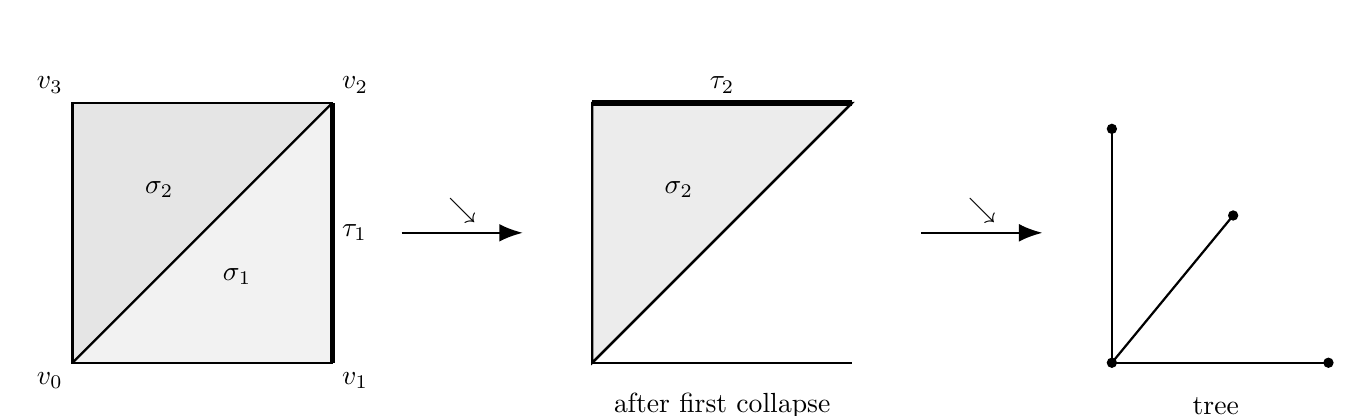
\begin{tikzpicture}[scale=1.1]
	% square
	\coordinate (A) at (0,0);
	\coordinate (B) at (3,0);
	\coordinate (C) at (3,3);
	\coordinate (D) at (0,3);
	
	\fill[gray!10] (A)--(B)--(C)--cycle;
	\fill[gray!20] (A)--(C)--(D)--cycle;
	
	\draw[thick] (A)--(B)--(C)--(D)--cycle;
	\draw[thick] (A)--(C);
	
	\node[below left] at (A) {$v_0$};
	\node[below right] at (B) {$v_1$};
	\node[above right] at (C) {$v_2$};
	\node[above left] at (D) {$v_3$};
	
	\draw[line width=2pt] (B)--(C);
	\node[right] at ($(B)!0.5!(C)$) {$\tau_1$};
	
	\node at (1.9,1.0) {$\sigma_1$};
	\node at (1.0,2.0) {$\sigma_2$};
	
	\draw[-{Latex[length=3mm]},thick] (3.8,1.5)--(5.2,1.5);
	\node[above] at (4.5,1.5) {$\searrow$};
	
	% after first collapse
	\begin{scope}[xshift=6cm]
		\coordinate (A) at (0,0);
		\coordinate (B) at (3,0);
		\coordinate (C) at (3,3);
		\coordinate (D) at (0,3);
		
		\fill[gray!15] (A)--(C)--(D)--cycle;
		\draw[thick] (A)--(B);
		\draw[thick] (A)--(C)--(D)--cycle;
		\draw[thick] (A)--(C);
		
		\draw[line width=2pt] (C)--(D);
		\node[above] at ($(C)!0.5!(D)$) {$\tau_2$};
		\node at (1.0,2.0) {$\sigma_2$};
		\node at (1.5,-0.5) {after first collapse};
	\end{scope}
	
	\draw[-{Latex[length=3mm]},thick] (9.8,1.5)--(11.2,1.5);
	\node[above] at (10.5,1.5) {$\searrow$};
	
	% final tree
	\begin{scope}[xshift=12cm]
		\coordinate (A) at (0,0);
		\coordinate (B) at (2.5,0);
		\coordinate (C) at (1.4,1.7);
		\coordinate (D) at (0,2.7);
		
		\draw[thick] (A)--(B);
		\draw[thick] (A)--(C);
		\draw[thick] (A)--(D);
		
		\filldraw (A) circle (1.5pt);
		\filldraw (B) circle (1.5pt);
		\filldraw (C) circle (1.5pt);
		\filldraw (D) circle (1.5pt);
		
		\node at (1.2,-0.5) {tree};
	\end{scope}
\end{tikzpicture}
\]

The remaining tree collapses to a point, so the whole square has the homology of a point.

\[
H_0(K)\cong \mathbb Z,
\qquad
H_j(K)=0
\quad
j\geq 1.
\]

\subsection{Diagram 5: Tree collapses by deleting leaf edges}

A tree collapses by repeatedly removing a leaf edge and its leaf vertex.

\[
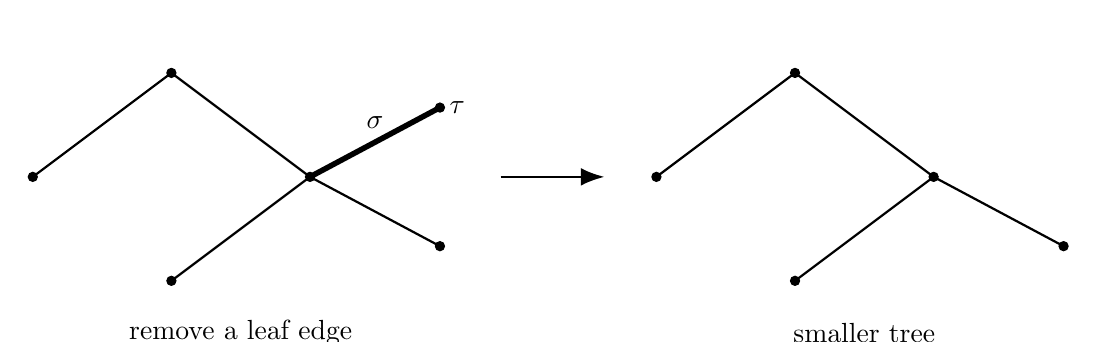
\begin{tikzpicture}[scale=1.1]
	% original tree
	\coordinate (A) at (0,0);
	\coordinate (B) at (1.6,1.2);
	\coordinate (C) at (3.2,0);
	\coordinate (D) at (1.6,-1.2);
	\coordinate (E) at (4.7,0.8);
	\coordinate (F) at (4.7,-0.8);
	
	\draw[thick] (A)--(B)--(C)--(D);
	\draw[thick] (C)--(E);
	\draw[thick] (C)--(F);
	
	\filldraw (A) circle (1.5pt);
	\filldraw (B) circle (1.5pt);
	\filldraw (C) circle (1.5pt);
	\filldraw (D) circle (1.5pt);
	\filldraw (E) circle (1.5pt);
	\filldraw (F) circle (1.5pt);
	
	\draw[line width=2pt] (C)--(E);
	\node[right] at (E) {$\tau$};
	\node[above] at (3.95,0.45) {$\sigma$};
	
	\node at (2.4,-1.8) {remove a leaf edge};
	
	\draw[-{Latex[length=3mm]},thick] (5.4,0)--(6.6,0);
	
	% smaller tree
	\begin{scope}[xshift=7.2cm]
		\coordinate (A) at (0,0);
		\coordinate (B) at (1.6,1.2);
		\coordinate (C) at (3.2,0);
		\coordinate (D) at (1.6,-1.2);
		\coordinate (F) at (4.7,-0.8);
		
		\draw[thick] (A)--(B)--(C)--(D);
		\draw[thick] (C)--(F);
		
		\filldraw (A) circle (1.5pt);
		\filldraw (B) circle (1.5pt);
		\filldraw (C) circle (1.5pt);
		\filldraw (D) circle (1.5pt);
		\filldraw (F) circle (1.5pt);
		
		\node at (2.4,-1.8) {smaller tree};
	\end{scope}
\end{tikzpicture}
\]

Repeating this process gives

\[
K\searrow \{\text{point}\}.
\]

\subsection{Diagram 6: Circle has no free vertex}

A triangulated circle has no free vertex, because every vertex belongs to two edges.

\[
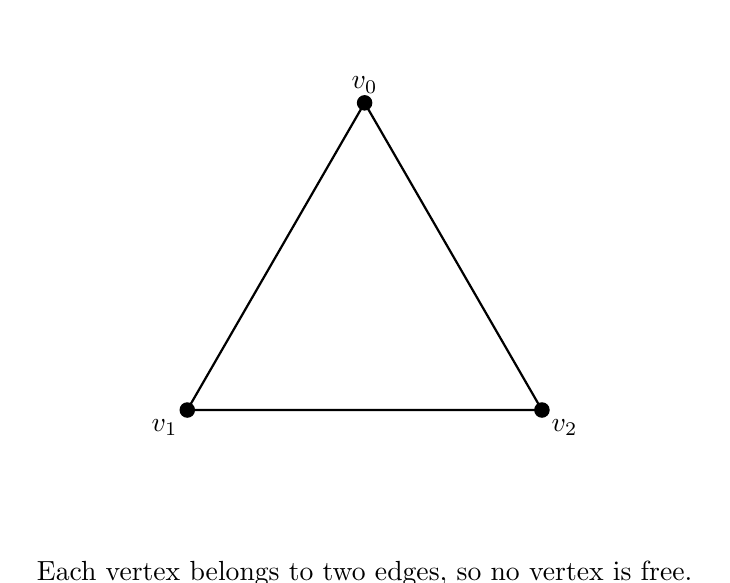
\begin{tikzpicture}[scale=1.3]
	\coordinate (A) at (90:2);
	\coordinate (B) at (210:2);
	\coordinate (C) at (330:2);
	
	\draw[thick] (A)--(B)--(C)--cycle;
	
	\filldraw (A) circle (2pt);
	\filldraw (B) circle (2pt);
	\filldraw (C) circle (2pt);
	
	\node[above] at (A) {$v_0$};
	\node[below left] at (B) {$v_1$};
	\node[below right] at (C) {$v_2$};
	
	\node at (0,-2.6) {Each vertex belongs to two edges, so no vertex is free.};
\end{tikzpicture}
\]

Therefore the circle cannot collapse to a point. Its homology is

\[
H_0(S^1)\cong \mathbb Z,
\qquad
H_1(S^1)\cong \mathbb Z.
\]

\subsection{Diagram 7: Annulus collapses to its central circle}

An annulus can be triangulated as a strip whose left and right sides are identified.

\[
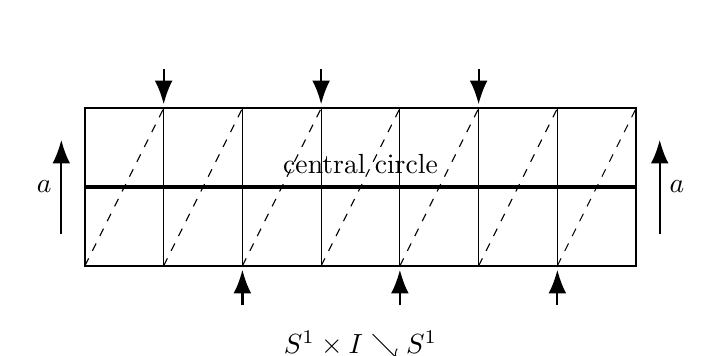
\begin{tikzpicture}[scale=1.0]
	% annulus strip
	\draw[thick] (0,0) rectangle (7,2);
	
	% vertical subdivisions
	\foreach \x in {1,2,3,4,5,6}{
		\draw[thin] (\x,0)--(\x,2);
	}
	
	% diagonals
	\foreach \x in {0,1,2,3,4,5,6}{
		\draw[thin,dashed] (\x,0)--(\x+1,2);
	}
	
	% boundary peeling arrows
	\draw[-{Latex[length=3mm]},thick] (1,2.5)--(1,2.05);
	\draw[-{Latex[length=3mm]},thick] (3,2.5)--(3,2.05);
	\draw[-{Latex[length=3mm]},thick] (5,2.5)--(5,2.05);
	
	\draw[-{Latex[length=3mm]},thick] (2,-0.5)--(2,-0.05);
	\draw[-{Latex[length=3mm]},thick] (4,-0.5)--(4,-0.05);
	\draw[-{Latex[length=3mm]},thick] (6,-0.5)--(6,-0.05);
	
	% side identifications
	\draw[-{Latex[length=3mm]},thick] (-0.3,0.4)--(-0.3,1.6);
	\draw[-{Latex[length=3mm]},thick] (7.3,0.4)--(7.3,1.6);
	
	\node[left] at (-0.3,1) {$a$};
	\node[right] at (7.3,1) {$a$};
	
	% central circle core
	\draw[very thick] (0,1)--(7,1);
	\node at (3.5,1.3) {central circle};
	
	\node at (3.5,-1.0) {$S^1\times I\searrow S^1$};
\end{tikzpicture}
\]

The annulus does not collapse to a point, because the central circle represents a genuine \(H_1\)-class:

\[
H_1(S^1\times I)\cong \mathbb Z.
\]

\subsection{Diagram 8: Filled tetrahedron versus boundary sphere}

A filled tetrahedron \(\Delta^3\) is collapsible. Its boundary \(\partial\Delta^3\cong S^2\) is not collapsible to a point.

\[
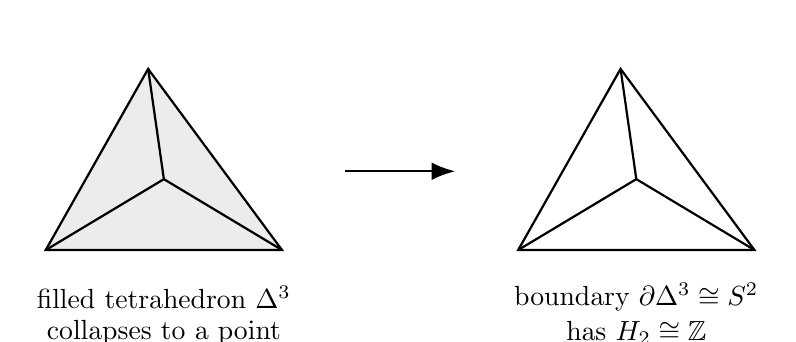
\begin{tikzpicture}[scale=1.0]
	% filled tetrahedron sketch
	\coordinate (A) at (0,0);
	\coordinate (B) at (3,0);
	\coordinate (C) at (1.3,2.3);
	\coordinate (D) at (1.5,0.9);
	
	\fill[gray!15] (A)--(B)--(C)--cycle;
	\draw[thick] (A)--(B)--(C)--cycle;
	\draw[thick] (A)--(D);
	\draw[thick] (B)--(D);
	\draw[thick] (C)--(D);
	\draw[dashed] (A)--(C);
	
	\node at (1.5,-0.6) {filled tetrahedron \(\Delta^3\)};
	\node at (1.5,-1.05) {collapses to a point};
	
	\draw[-{Latex[length=3mm]},thick] (3.8,1)--(5.2,1);
	
	% boundary sphere sketch
	\begin{scope}[xshift=6cm]
		\coordinate (A) at (0,0);
		\coordinate (B) at (3,0);
		\coordinate (C) at (1.3,2.3);
		\coordinate (D) at (1.5,0.9);
		
		\draw[thick] (A)--(B)--(C)--cycle;
		\draw[thick] (A)--(D);
		\draw[thick] (B)--(D);
		\draw[thick] (C)--(D);
		
		\node at (1.5,-0.6) {boundary \(\partial\Delta^3\cong S^2\)};
		\node at (1.5,-1.05) {has \(H_2\cong\mathbb Z\)};
	\end{scope}
\end{tikzpicture}
\]

The filled tetrahedron has

\[
H_0\cong \mathbb Z,
\qquad
H_j=0
\quad
j\geq 1.
\]

The boundary sphere has

\[
H_0(S^2)\cong \mathbb Z,
\qquad
H_2(S^2)\cong \mathbb Z.
\]

\subsection{Diagram 9: Chain cancellation picture}

An elementary collapse removes an acyclic two-term chain piece:

\[
\mathbb Z[\sigma]\xrightarrow{\cong}\mathbb Z[\tau].
\]

\[
\begin{tikzcd}[column sep=large,row sep=large]
	0
	\arrow[r]
	&
	\mathbb Z[\sigma]
	\arrow[r,"\partial"]
	&
	\mathbb Z[\tau]
	\arrow[r]
	&
	0
	\\
	&
	\sigma
	\arrow[r,mapsto]
	&
	\tau
	&
\end{tikzcd}
\]

Since this relative complex has zero homology, removing \(\sigma\) and \(\tau\) preserves the homology of the whole complex.

\subsection{Chart 1: What collapses and what does not collapse}

\[
\begin{array}{c|c|c|c}
	\text{Complex} & \text{Free face exists?} & \text{Collapse result} & \text{Homology} \\
	\hline
	\text{interval}
	&
	\text{yes}
	&
	\text{point}
	&
	H_0\cong \mathbb Z
	\\
	\hline
	\text{filled triangle}
	&
	\text{yes}
	&
	\text{point}
	&
	H_0\cong \mathbb Z
	\\
	\hline
	\text{tree}
	&
	\text{yes, leaf vertices}
	&
	\text{point}
	&
	H_0\cong \mathbb Z
	\\
	\hline
	\text{circle}
	&
	\text{no}
	&
	\text{does not collapse to point}
	&
	H_0\cong \mathbb Z,\ H_1\cong \mathbb Z
	\\
	\hline
	\text{annulus}
	&
	\text{yes on boundary}
	&
	S^1
	&
	H_0\cong \mathbb Z,\ H_1\cong \mathbb Z
	\\
	\hline
	\text{filled tetrahedron}
	&
	\text{yes}
	&
	\text{point}
	&
	H_0\cong \mathbb Z
	\\
	\hline
	\partial\Delta^3\cong S^2
	&
	\text{no 2-dimensional free face}
	&
	\text{does not collapse to point}
	&
	H_0\cong \mathbb Z,\ H_2\cong \mathbb Z
	\\
	\hline
	T^2
	&
	\text{no collapse to point}
	&
	\text{obstructed by homology}
	&
	H_0\cong \mathbb Z,\ H_1\cong \mathbb Z^2,\ H_2\cong \mathbb Z
\end{array}
\]

\subsection{Chart 2: Collapse versus homology}

\[
\begin{array}{c|c|c}
	\text{Situation} & \text{Geometric meaning} & \text{Homological meaning} \\
	\hline
	\text{free face exists}
	&
	\text{a simplex is attached in a removable way}
	&
	\text{acyclic cancellation pair}
	\\
	\hline
	K\searrow L
	&
	\text{remove }(\sigma,\tau)
	&
	H_j(K)\cong H_j(L)
	\\
	\hline
	K\searrow \text{point}
	&
	\text{complex is collapsible}
	&
	H_0\cong \mathbb Z,\ H_j=0\text{ for }j\geq 1
	\\
	\hline
	\text{no free face}
	&
	\text{nothing removable by collapse}
	&
	\text{may contain genuine cycles}
	\\
	\hline
	H_1\neq 0
	&
	\text{loop exists}
	&
	\text{cannot collapse to a point}
	\\
	\hline
	H_2\neq 0
	&
	\text{closed surface exists}
	&
	\text{cannot collapse to a point}
\end{array}
\]

\subsection{Final visual summary}


\[
\begin{tikzcd}[column sep=large,row sep=large]
	K
	\arrow[r, "{\mathrm{remove\ free\ pair}\ (\sigma,\tau)}"]
	\arrow[dr, swap, "{H_j(K)}"]
	&
	L=K\setminus\{\sigma,\tau\}
	\arrow[d, "{H_j(L)}"]
	\\
	& H_j(K)\cong H_j(L)
\end{tikzcd}
\]


The essential idea is:

\[
\boxed{
	\text{Elementary collapse removes an acyclic piece, so homology is unchanged.}
}
\]

% ============================================================
% Deep theory for Problems 4 and 5 (Algebraic Topology / 4-manifolds)
% Self-contained LaTeX section.
% Requires: amsmath, amssymb, amsthm, mathtools.
% ============================================================

\section{Deep theory for Problems 4--5: connected sums, intersection forms, and parity phenomena}

\subsection{Problem 4: same homology, not homotopy equivalent}

We consider the closed oriented $4$-manifolds
\[
X_1=\CP^2\#\CP^2,\qquad
X_2=\CP^2\#\overline{\CP^2},\qquad
X_3=S^2\times S^2,
\]
and we want to understand why
\[
H_*(X_1)\cong H_*(X_2)\cong H_*(X_3)
\]
as graded abelian groups, while no two of the $X_i$ are homotopy equivalent.

\subsubsection{A. Homology of a connected sum in dimension $n\ge 3$}

Let $M$ and $N$ be closed connected $n$-manifolds with $n\ge 3$. Remove the interior of an embedded $n$-ball from each and glue along the boundary sphere:
\[
M\# N := (M\setminus \operatorname{int}D^n)\cup_{S^{n-1}}(N\setminus \operatorname{int}D^n).
\]
Write $M^\circ:=M\setminus \operatorname{int}D^n$ and $N^\circ:=N\setminus \operatorname{int}D^n$, so that
\[
M\# N = M^\circ \cup N^\circ,\qquad M^\circ\cap N^\circ \cong S^{n-1}.
\]
Applying Mayer--Vietoris to $(M^\circ, N^\circ)$ and using $H_i(S^{n-1})=0$ for $0<i<n-1$ yields the standard conclusion:
\[
H_i(M\#N)\cong H_i(M)\oplus H_i(N)\quad \text{for }1\le i\le n-2.
\]
In the top degrees one still has
\[
H_0(M\#N)\cong \mathbb Z,\qquad H_n(M\#N)\cong \mathbb Z,
\]
and the behavior in degree $n-1$ can be analyzed similarly (in our applications below, $n=4$ so $n-1=3$ and the groups are typically $0$ anyway).

\subsubsection{B. Apply to $X_1,X_2,X_3$}

Recall:
\[
H_*(\CP^2)\;:\quad H_0\cong \mathbb Z,\; H_2\cong \mathbb Z,\; H_4\cong \mathbb Z,\;\text{others }0,
\]
and orientation reversal does not change homology groups:
\[
H_*(\overline{\CP^2})\cong H_*(\CP^2).
\]
Also
\[
H_*(S^2\times S^2)\;:\quad H_0\cong \mathbb Z,\; H_2\cong \mathbb Z^2,\; H_4\cong \mathbb Z,\;\text{others }0.
\]

Using the connected-sum homology rule for $n=4$ (so for $i=1,2$ we get direct sums, and in these examples $H_1=H_3=0$), we obtain:
\[
H_2(\CP^2\#\CP^2)\cong \mathbb Z\oplus \mathbb Z\cong \mathbb Z^2,
\]
\[
H_2(\CP^2\#\overline{\CP^2})\cong \mathbb Z\oplus \mathbb Z\cong \mathbb Z^2,
\]
and of course $H_0\cong \mathbb Z$, $H_4\cong \mathbb Z$, and $H_1=H_3=0$ for all three. Hence
\[
H_*(X_1)\cong H_*(X_2)\cong H_*(X_3)
\]
as graded abelian groups.

\subsubsection{C. Why homology does \emph{not} determine homotopy type in dimension $4$}

For a closed oriented $4$-manifold $X$, the key additional invariant is the \emph{intersection form} on middle cohomology:
\[
Q_X: H^2(X;\mathbb Z)/\text{tors} \times H^2(X;\mathbb Z)/\text{tors}\longrightarrow \mathbb Z,
\qquad
Q_X(\alpha,\beta)=\langle \alpha\smile \beta, [X]\rangle.
\]
This is a unimodular symmetric bilinear form (unimodular meaning the induced map to the dual lattice is an isomorphism).

\begin{remark}[Homotopy invariance]
	A homotopy equivalence $f:X\to Y$ induces a ring isomorphism
	\[
	f^*:H^*(Y;\mathbb Z)\xrightarrow{\ \cong\ } H^*(X;\mathbb Z),
	\]
	and it sends $[Y]$ to $\pm [X]$ in top degree. Therefore $f^*$ identifies the cup product pairings, and in particular identifies the intersection forms up to change of $\mathbb Z$-basis (integral congruence). Thus:
	\[
	X\simeq Y \;\Longrightarrow\; Q_X \cong Q_Y \text{ (as integral forms, up to sign depending on orientation).}
	\]
\end{remark}

\subsubsection{D. Behavior under connected sum and orientation reversal}

Two fundamental structural facts:
\begin{itemize}
	\item (\textbf{Connected sum}) For oriented $4$-manifolds,
	\[
	Q_{X\#Y}\;\cong\; Q_X \oplus Q_Y.
	\]
	\item (\textbf{Orientation reversal}) If $\overline{X}$ is $X$ with reversed orientation, then
	\[
	Q_{\overline{X}} \cong -\,Q_X.
	\]
\end{itemize}

\subsubsection{E. Compute $Q$ for the three examples}

\paragraph{1. The form of $\CP^2$.}
Let $a\in H^2(\CP^2;\mathbb Z)$ be the standard generator (hyperplane class). Then
\[
\langle a\smile a, [\CP^2]\rangle = 1,
\]
so
\[
Q_{\CP^2}=[1].
\]
Hence
\[
Q_{\overline{\CP^2}}=[-1].
\]

\paragraph{2. The form of $X_1=\CP^2\#\CP^2$.}
By direct sum:
\[
Q_{X_1}\cong [1]\oplus[1].
\]
This form is \emph{positive definite} and has signature $+2$.

\paragraph{3. The form of $X_2=\CP^2\#\overline{\CP^2}$.}
\[
Q_{X_2}\cong [1]\oplus[-1].
\]
This form is \emph{indefinite} with signature $0$, and it is \emph{odd} (since it has a vector of square $1$).

\paragraph{4. The form of $X_3=S^2\times S^2$.}
Let $u=[S^2\times\{\ast\}]^\vee$ and $v=[\{\ast\}\times S^2]^\vee$ be the standard basis of $H^2(S^2\times S^2;\mathbb Z)\cong \mathbb Z^2$. Then
\[
u\smile u = 0,\quad v\smile v=0,\quad u\smile v \text{ evaluates to }1 \text{ on }[S^2\times S^2],
\]
so in the basis $(u,v)$ we have
\[
Q_{S^2\times S^2}\cong
\begin{pmatrix}
	0 & 1\\
	1 & 0
\end{pmatrix}.
\]
This form is \emph{indefinite} with signature $0$, and it is \emph{even} (every vector has even self-intersection).

\subsubsection{F. Separate the homotopy types}

We now compare invariants of the forms:
\begin{itemize}
	\item $Q_{X_1}$ is \emph{definite} (signature $+2$), while $Q_{X_2}$ and $Q_{X_3}$ are \emph{indefinite} (signature $0$). Therefore $X_1$ is not homotopy equivalent to $X_2$ or $X_3$.
	\item $Q_{X_2}$ is \emph{odd}, while $Q_{X_3}$ is \emph{even}. Therefore $X_2$ is not homotopy equivalent to $X_3$.
\end{itemize}
Hence no two of $X_1,X_2,X_3$ are homotopy equivalent, despite having the same homology groups.

\begin{remark}[Takeaway]
	Homology groups alone do not determine the homotopy type of a closed oriented $4$-manifold. The \emph{cup product structure} in degree $2$ (equivalently, the intersection form) is a strictly finer invariant and is preserved by homotopy equivalence.
\end{remark}

% ------------------------------------------------------------

\subsection{Problem 5: parity of the middle Betti number in dimension $4n+2$}

Let $M$ be a closed $\mathbb Z$-orientable manifold of dimension $4n+2$. We show that
\[
\dim_{\mathbb Q} H_{2n+1}(M;\mathbb Q) \text{ is even.}
\]

\subsubsection{A. Poincar\'e duality gives a perfect middle pairing}

Since $M$ is $\mathbb Z$-orientable, it is also $\mathbb Q$-orientable, and Poincar\'e duality gives a perfect pairing
\[
H^{k}(M;\mathbb Q)\times H^{(4n+2)-k}(M;\mathbb Q)\longrightarrow \mathbb Q,
\qquad
(\alpha,\beta)\mapsto \langle \alpha\smile \beta,[M]\rangle.
\]
In particular, when $k=2n+1$ we obtain a bilinear pairing on the \emph{same} vector space:
\[
\langle \cdot,\cdot\rangle \;:\; H^{2n+1}(M;\mathbb Q)\times H^{2n+1}(M;\mathbb Q)\to \mathbb Q,
\qquad
\langle \alpha,\beta\rangle=\langle \alpha\smile\beta,[M]\rangle,
\]
and Poincar\'e duality implies this pairing is nondegenerate.

\subsubsection{B. Graded commutativity forces skew-symmetry}

The cup product is graded-commutative:
\[
\alpha\smile\beta = (-1)^{|\alpha||\beta|}\,\beta\smile\alpha.
\]
Here $|\alpha|=|\beta|=2n+1$ is odd, hence $|\alpha||\beta|$ is odd and
\[
\alpha\smile\beta = -\,\beta\smile\alpha.
\]
Therefore the pairing satisfies
\[
\langle \alpha,\beta\rangle = -\,\langle \beta,\alpha\rangle,
\]
so it is \emph{skew-symmetric}. Over $\mathbb Q$ (characteristic $\neq 2$), skew-symmetry implies
\[
\langle \alpha,\alpha\rangle = 0 \qquad \text{for all }\alpha.
\]
Thus the pairing is an \emph{alternating} nondegenerate bilinear form.

\subsubsection{C. Linear algebra lemma: nondegenerate alternating forms have even dimension}

\begin{lemma}[Symplectic dimension parity]
	Let $V$ be a finite-dimensional vector space over a field of characteristic $\neq 2$, and let
	$\omega:V\times V\to \Bbbk$ be a nondegenerate alternating bilinear form. Then $\dim V$ is even.
\end{lemma}

\begin{proof}
	Over such a field, one can build a symplectic basis by induction: choose $v\neq 0$, then nondegeneracy gives $w$ with $\omega(v,w)\neq 0$, and $\langle v,w\rangle$ is a $2$-dimensional nondegenerate subspace; take its orthogonal complement and continue. Hence $V$ decomposes into a direct sum of $2$-dimensional symplectic blocks, so $\dim V$ is even.
\end{proof}

Applying the lemma to
\[
V=H^{2n+1}(M;\mathbb Q)
\]
with $\omega(\alpha,\beta)=\langle \alpha\smile\beta,[M]\rangle$ yields:
\[
\dim_{\mathbb Q} H^{2n+1}(M;\mathbb Q)\ \text{is even.}
\]

\subsubsection{D. Convert to homology}

Over a field, universal coefficients gives
\[
H^{2n+1}(M;\mathbb Q)\cong \Hom(H_{2n+1}(M;\mathbb Q),\mathbb Q),
\]
so
\[
\dim_{\mathbb Q} H^{2n+1}(M;\mathbb Q)=\dim_{\mathbb Q} H_{2n+1}(M;\mathbb Q).
\]
Therefore $\dim_{\mathbb Q} H_{2n+1}(M;\mathbb Q)$ is even, as desired.

\begin{remark}[Interpretation]
	In dimension $4n+2$, the middle cup-product pairing is symplectic (alternating) rather than symmetric, forcing the middle Betti number to come in pairs.
\end{remark}

% ============================================================
% Examples for Problem 5 (middle Betti number even in dim 4n+2)
% Paste after your theory section.
% ============================================================

\subsection{Examples for Problem 5: evenness of the middle Betti number in dimension \(4n+2\)}

Recall the statement: if \(M\) is a closed \(\mathbb Z\)-orientable manifold of dimension \(4n+2\),
then
\[
\dim_{\mathbb Q} H_{2n+1}(M;\mathbb Q)\ \text{is even}.
\]
Equivalently, the middle Betti number \(b_{2n+1}(M)\) is even (over \(\mathbb Q\)).

\subsubsection{Example 1: Closed oriented surfaces \(\Sigma_g\) (the case \(n=0\))}

Here \(\dim \Sigma_g = 2 = 4\cdot 0 + 2\), so the relevant group is \(H_1(\Sigma_g;\mathbb Q)\).
We have the classical computation:
\[
H_0(\Sigma_g;\mathbb Q)\cong \mathbb Q,\qquad
H_1(\Sigma_g;\mathbb Q)\cong \mathbb Q^{2g},\qquad
H_2(\Sigma_g;\mathbb Q)\cong \mathbb Q.
\]
Hence
\[
\dim_{\mathbb Q} H_1(\Sigma_g;\mathbb Q)=2g,
\]
which is even, as predicted. The cup product pairing on \(H^1(\Sigma_g;\mathbb Q)\) is the standard
nondegenerate skew-symmetric (symplectic) intersection pairing.

\subsubsection{Example 2: \(\Sigma_g\times S^4\) (dimension \(6\), i.e. \(n=1\))}

Let
\[
M=\Sigma_g\times S^4.
\]
Then \(\dim M = 2+4=6=4\cdot 1+2\), so the middle degree is \(2n+1=3\).
Using K\"unneth over \(\mathbb Q\),
\[
H_3(\Sigma_g\times S^4;\mathbb Q)
\cong
H_3(\Sigma_g;\mathbb Q)\otimes H_0(S^4;\mathbb Q)
\ \oplus\
H_1(\Sigma_g;\mathbb Q)\otimes H_2(S^4;\mathbb Q)
\ \oplus\
H_0(\Sigma_g;\mathbb Q)\otimes H_3(S^4;\mathbb Q).
\]
But
\[
H_3(\Sigma_g;\mathbb Q)=0,\quad H_2(S^4;\mathbb Q)=0,\quad H_3(S^4;\mathbb Q)=0,
\]
so
\[
H_3(\Sigma_g\times S^4;\mathbb Q)=0,
\]
and therefore \(\dim H_3=0\), which is even.

\subsubsection{Example 3: \(S^3\times S^3\) (dimension \(6\), i.e. \(n=1\))}

Let
\[
M=S^3\times S^3.
\]
Then \(\dim M=6\) and the middle degree is \(3\).
By K\"unneth over \(\mathbb Q\),
\[
H_3(S^3\times S^3;\mathbb Q)
\cong
H_3(S^3;\mathbb Q)\otimes H_0(S^3;\mathbb Q)
\ \oplus\
H_0(S^3;\mathbb Q)\otimes H_3(S^3;\mathbb Q)
\cong
\mathbb Q\oplus \mathbb Q.
\]
Hence
\[
\dim_{\mathbb Q} H_3(S^3\times S^3;\mathbb Q)=2,
\]
which is even. In this example the middle cohomology pairing is a \(2\times 2\) skew form.

\subsubsection{Example 4: Connected sums \(\#^k(S^3\times S^3)\) (dimension \(6\))}

Let
\[
M=\#^k(S^3\times S^3).
\]
Then \(M\) is closed oriented of dimension \(6\), and the middle degree is \(3\).
For connected sums in dimension \(\ge 3\),
\[
H_3\!\left(\#^k(S^3\times S^3);\mathbb Q\right)
\cong
\bigoplus_{j=1}^k H_3(S^3\times S^3;\mathbb Q)
\cong
(\mathbb Q^2)^{\oplus k}\cong \mathbb Q^{2k}.
\]
Thus
\[
\dim_{\mathbb Q} H_3(M;\mathbb Q)=2k,
\]
again even. This gives a large family where the middle Betti number can be any even integer.

\subsubsection{Example 5: Products \(\Sigma_g\times S^{4n}\) (general \(n\ge 1\))}

Let \(n\ge 1\) and set
\[
M=\Sigma_g\times S^{4n}.
\]
Then \(\dim M=2+4n=4n+2\), and the middle degree is \(2n+1\).
By K\"unneth over \(\mathbb Q\),
\[
H_{2n+1}(M;\mathbb Q)
\cong
\bigoplus_{i+j=2n+1} H_i(\Sigma_g;\mathbb Q)\otimes H_j(S^{4n};\mathbb Q).
\]
But the only nonzero rational homology of \(S^{4n}\) is in degrees \(0\) and \(4n\), so the only possible
summands would require \(j=0\) or \(j=4n\), i.e.
\[
i=2n+1 \quad \text{or}\quad i=2n+1-4n=1-2n.
\]
For \(n\ge 1\), both indices are impossible for \(\Sigma_g\) (the first is \(>2\), the second is negative), so
\[
H_{2n+1}(\Sigma_g\times S^{4n};\mathbb Q)=0.
\]
Hence the middle Betti number is \(0\), which is even.

\subsubsection{Remark: why orientability matters and why \(\mathbb F_2\) is different}

The evenness argument uses a nondegenerate \emph{alternating} pairing on \(H^{2n+1}(M;\mathbb Q)\).
Over a field of characteristic \(2\), “skew-symmetric” and “symmetric” coincide, and one can no longer
conclude that the dimension must be even. This is why the clean parity statement is formulated over
\(\mathbb Q\) (or any field of characteristic \(\neq 2\)).

% ============================================================
% Orientability dictionary: closed / orientable / Z-orientable / Q-orientable
% ============================================================

\subsection{Closed and orientable vs.\ \(\mathbb Z\)-orientable and \(\mathbb Q\)-orientable}

\subsubsection{Closed manifolds}
An \(n\)-manifold \(M\) is \textbf{closed} if it is \emph{compact} and has \emph{empty boundary}:
\[
M \text{ closed}\quad \Longleftrightarrow\quad M \text{ compact and }\partial M=\varnothing.
\]
Examples: \(S^n\), \(T^n\), \(\mathbb{CP}^m\).
Non-examples: \(D^n\) (has boundary), \(\mathbb R^n\) (not compact).

\subsubsection{Orientable manifolds}
A manifold \(M\) is \textbf{orientable} if one can choose a consistent orientation on all coordinate
charts (equivalently, all transition maps between oriented charts have positive Jacobian determinant in the smooth case).
There are several equivalent algebraic-topological characterizations.

\begin{remark}[Homology characterization for closed connected manifolds]
	If \(M\) is a connected closed \(n\)-manifold, then
	\[
	M \text{ orientable}\quad \Longleftrightarrow\quad H_n(M;\mathbb Z)\cong \mathbb Z,
	\]
	and
	\[
	M \text{ nonorientable}\quad \Longleftrightarrow\quad H_n(M;\mathbb Z)=0.
	\]
\end{remark}

\subsubsection{\(\mathbb Z\)-orientable}
Saying that \(M\) is \textbf{\(\mathbb Z\)-orientable} means that \(M\) admits a fundamental class with integer coefficients.
For a connected closed \(n\)-manifold this is exactly the usual notion of orientability:
\[
\mathbb Z\text{-orientable}\quad \Longleftrightarrow\quad \text{orientable}.
\]

\subsubsection{\(F\)-orientable and \(\mathbb Q\)-orientable}
Let \(F\) be a field. A connected closed \(n\)-manifold \(M\) is called \textbf{\(F\)-orientable} if it admits a fundamental class
\([M]_F\in H_n(M;F)\), equivalently
\[
H_n(M;F)\cong F.
\]
In particular, \(M\) is \textbf{\(\mathbb Q\)-orientable} if
\[
H_n(M;\mathbb Q)\cong \mathbb Q.
\]

\begin{remark}[Relations between \(\mathbb Z\)- and \(\mathbb Q\)-orientability]
	For closed connected manifolds one has
	\[
	\mathbb Z\text{-orientable}\ \Longrightarrow\ \mathbb Q\text{-orientable}.
	\]
	Moreover, since \(\mathbb Q\) has characteristic \(\neq 2\), for manifolds one actually has the equivalence
	\[
	\mathbb Q\text{-orientable}\ \Longleftrightarrow\ \mathbb Z\text{-orientable}\ \Longleftrightarrow\ \text{orientable}.
	\]
\end{remark}

\subsubsection{The special role of \(\mathbb F_2\)}
Over the field \(\mathbb F_2\), signs disappear (\(-1=+1\)), and every manifold becomes orientable.

\begin{remark}[\(\mathbb F_2\)-orientability]
	Every connected closed manifold \(M\) is \(\mathbb F_2\)-orientable:
	\[
	H_n(M;\mathbb F_2)\cong \mathbb F_2.
	\]
	For example, \(\mathbb{RP}^2\) is not \(\mathbb Z\)-orientable (so \(H_2(\mathbb{RP}^2;\mathbb Z)=0\)),
	but it is \(\mathbb F_2\)-orientable (so \(H_2(\mathbb{RP}^2;\mathbb F_2)\cong \mathbb F_2\)).
\end{remark}

\subsubsection{Why this matters for Poincar\'e duality}
Let \(M\) be a connected closed \(n\)-manifold and let \(F\) be a field.
If \(M\) is \(F\)-orientable, then Poincar\'e duality holds with coefficients in \(F\):
\[
H^i(M;F)\cong H_{n-i}(M;F),
\]
via cap product with the fundamental class \([M]_F\).
In particular:
\begin{itemize}
	\item If \(M\) is orientable, then duality holds over \emph{any} field \(F\) (including \(\mathbb Q\)).
	\item For an arbitrary (possibly nonorientable) manifold, duality always holds over \(\mathbb F_2\).
\end{itemize}

\subsubsection{Summary}
For connected closed manifolds:
\[
\text{orientable}\ \Longleftrightarrow\ \mathbb Z\text{-orientable}\ \Longleftrightarrow\ \mathbb Q\text{-orientable},
\]
while
\[
\text{every manifold is } \mathbb F_2\text{-orientable}.
\]



\end{document}



